\documentclass[12pt]{report}
\usepackage[T1]{fontenc}
\usepackage[utf8]{inputenc}
\usepackage{caption}
\usepackage{adjustbox}
\usepackage{graphicx}
\usepackage{amsmath,amssymb,amsfonts}
\usepackage{txfonts}
\usepackage{listings}
\usepackage{float}
\usepackage{color}
\usepackage{xcolor}
\usepackage{enumitem}
\graphicspath{{images/}}
\renewcommand{\chaptername}{Rozdział}
\renewcommand{\contentsname}{Spis treści}
\renewcommand{\figurename}{Rysunek}
\renewcommand{\listfigurename}{Spis rysunków}
\renewcommand{\bibname}{Bibliografia}
\setlength{\textwidth}{14cm}
\setlength{\textheight}{20cm}
\newtheorem{definition}{Definicja}
\newtheorem{example}{Przykład}[chapter] 
\newtheorem{corollary}{Wniosek}[chapter]

\lstdefinelanguage{JavaScript}{
  keywords={typeof, new, true, false, catch, function, return, null, catch, switch, var, if, in, while, do, else, case, break},
  keywordstyle=\color{blue}\bfseries,
  ndkeywords={class, export, boolean, throw, implements, import, this},
  ndkeywordstyle=\color{darkgray}\bfseries,
  identifierstyle=\color{black},
  sensitive=false,
  comment=[l]{//},
  morecomment=[s]{/*}{*/},
  commentstyle=\color{purple}\ttfamily,
  stringstyle=\color{red}\ttfamily,
  morestring=[b]',
  morestring=[b]"
}

\lstset{
   language=JavaScript,
   backgroundcolor=\color{lightgray},
   extendedchars=true,
   basicstyle=\footnotesize\ttfamily,
   showstringspaces=false,
   showspaces=false,
   numbers=left,
   numberstyle=\footnotesize,
   numbersep=9pt,
   tabsize=2,
   breaklines=true,
   showtabs=false,
   captionpos=b
}

\lstdefinelanguage{XML}
{
  morestring=[b]",
  morestring=[s]{>}{<},
  morecomment=[s]{<?}{?>},
  stringstyle=\color{black},
  identifierstyle=\color{blue},
  keywordstyle=\color{cyan},
  morekeywords={xmlns,version,type}% list your attributes here
}

\lstset{
  basicstyle=\ttfamily,
  columns=fullflexible,
  showstringspaces=false,
  commentstyle=\color{gray}\upshape
}

\colorlet{punct}{red!60!black}
\definecolor{background}{HTML}{EEEEEE}
\definecolor{lightgray}{rgb}{.9,.9,.9}
\definecolor{darkgray}{rgb}{.4,.4,.4}
\definecolor{purple}{rgb}{0.65, 0.12, 0.82}
\definecolor{delim}{RGB}{20,105,176}
\colorlet{numb}{magenta!60!black}

\lstdefinelanguage{json}{
    basicstyle=\normalfont\ttfamily,
    numbers=left,
    numberstyle=\scriptsize,
    stepnumber=1,
    numbersep=8pt,
    showstringspaces=false,
    breaklines=true,
    frame=lines,
    backgroundcolor=\color{background},
    literate=
     *{0}{{{\color{numb}0}}}{1}
      {1}{{{\color{numb}1}}}{1}
      {2}{{{\color{numb}2}}}{1}
      {3}{{{\color{numb}3}}}{1}
      {4}{{{\color{numb}4}}}{1}
      {5}{{{\color{numb}5}}}{1}
      {6}{{{\color{numb}6}}}{1}
      {7}{{{\color{numb}7}}}{1}
      {8}{{{\color{numb}8}}}{1}
      {9}{{{\color{numb}9}}}{1}
      {:}{{{\color{punct}{:}}}}{1}
      {,}{{{\color{punct}{,}}}}{1}
      {\{}{{{\color{delim}{\{}}}}{1}
      {\}}{{{\color{delim}{\}}}}}{1}
      {[}{{{\color{delim}{[}}}}{1}
      {]}{{{\color{delim}{]}}}}{1},
}

\begin{document}
\begin{titlepage}
	\centering
	{\scshape\LARGE Celem pracy jest przedstawienie technologii Node.js na przykładzie zaprojektowaniej aplikacji przeznaczonej do zarządzania codziennymi zadaniami.  \par}
\end{titlepage}
\tableofcontents

\chapter{Przedstawienie ogólne, ideologii oraz przeznaczenia technologii Node.js}

\section{Wstęp}
Node.js czyli cross-platformowy, działający niezależnie od środowiska język programowania napisany w jezykach c/c++ oraz javascript wydany 27 marca 2009 roku, zaprojektowany przez Ryan’a Dahl’a. 
Pozwala na tworzenie serwerów i narzędzi sieciowych działających po stronie serwera. 
Przed powstaniem języka kod javascriptowy był wykonywany głównie przez przegladarke internetową po stronie klienta, co pozwalało na bezproblemowa manipulacje kodem źródłowym strony przez użytkownika dając możliwość wykonywania złośliwych skryptów, naruszenie bezpieczenstwa baz danych lub uzyskania dostępu do chronionych zasobów servera. 
Środowisko Node.js może działać niezależnie od środowiska uruchomieniowego. 
Jest ono zgode z wieloma systemami operacyjnymi jak  Linux, macOS, Microsoft Windows, NonStop, czy serwerami Unix. 
Język ten cieszy się duża popularnością oraz pozytywnym odbiorem wśród użytkowników dzięki czemu mimo względnie krótkiego okresu życia środowiska zaowocowało ogromną ilością projektów open-source, tysiącami członków należących do społeczności okołojęzykowej oraz powstaniem wydarzeń poruszających tematy okołośrodowiskowe takimi jak NodeConf, Node Interactive lub Node Summit. 
Obecnie wiele największych firm korzysta z serwerów napisanych w języku Node.js. 
Ich przykładami są między innymi Groupon, IBM, Linkedln, Microsoft, Netflix, PayPal, Yahoo. 
Najpopularniejszymi API wspierającymi edycję oraz debugowanie kodu Node.js są Atom, Brackets, JetBrains, Microsoft Visual Studio, NetBeans czy Nodeclipse.

\section{Przeznaczenie}
Node.js zalecany jest do tworzenia aplikacji: 
\begin{itemize}
\item z dużą liczbą operacji wejścia/wyjścia,
\item strumieniowania danych np. video, 
\item Single Page Applications (SPA),
\item udostępniających API w formacie JSON,
\item z intensywną wymianą danych w czasie rzeczywistym na wielu urządzeniach np. portale społecznościowe.
\end{itemize} 
Ponieważ jest on szybki i lekki, może być stosowany do pisania między innymi bramki API. 
API to skrót od Application Programming Interface; opisuje jak poszczególne elementy lub warstwy oprogramowania powinny się komunikować. 
W praktyce to najczęściej biblioteka oferująca metody, które umożliwiają realizację określonych zadań. 
Node.js pozwala na zoptymalizowanie pracy oraz uzyskanie skalowalnosci dzięki asynchronicznemu przetwarzaniu danych dostarczanych do aplikacji w związku z czym idealnie nadaje sie do obsługi komunikacji wymagającej pracy w czasie rzeczywistym. 
Funkcje napisane w Node.js wykonują się równolegle, korzystajac z tak zwanych wywołań zwrotnych (ang. callback), przeciwnie jak w językach takich jak np. php gdzie program jest wykonywany synchronicznie - linia po lini. 
Dzięki temu nie powstaję problem blokowania określonych funkcjonalności programu w czasie pracy innych niezależnych jego części. 
Przy pomocy wywołań zwrotnych możemy zapewnić zasygnalizowanie uzyskanych wyników lub zwrócenie, bądź obsługe błędu powstałego w czasie działania bloku kodu.

\section{Modułowość}
Praca z Node.js opiera się głównie o korzystanie ze zbioru zdefiniowanych w ramach modułów funkcji wspierających określone funkcjonalności. 
Zapewniają one prace między innymi z plikami systemowymi, z urządzeniami wejścia/wyjścia, protokołami internetowymi (dns, http, tcp, tls/ssl, udp), plikami binarnymi, źródłami danych oraz funckjami kryptograficznymi. 
Zmiejszają one złożoność, a co za tym idzie nakład pracy przy tworzeniu własnej funkcjonalności. 
Dzięki wsparciu package managera (od roku 2010) nazywanego npm programiści mogą bez przeszkód udostępniać napisane przez siebie moduły i biblioteki lub w prosty sposób zainportowywać ogólnie dostępne moduły i używac ich w swoich projektach. 
Najpopularniejszymi modułami wykorzystywanymi w celu poprawy jakości oraz zmiejszenia nakładów pracy przy wytwarzaniu oprogramowania są Express.js, Socket.IO, Hapi.js, Sails.js czy Meteor. 
Npm jest automatycznie właczony w środowisko Node.js. 
Jest obsługiwany za pomocą lini komend systemu operacyjnego. 
Moduły są zapisane w formacie CommonJS oraz zawierają pliki informacyjne w formacie Json. 
Ilość ogólno dostępnych modułów przekracza obecnie 477000. 
Jest to spowodowane możliwością przez każdego użytkownika Node.js, bez potrezby wcześniejszej rejerstracji czy przejścia jakiejkolwiek procedury wstępnej udostepnienia napisanego przez siebie kodu. 
W związku z tym, wiele dostępnych modułów jest niskiej jakości, może zawierać elementy złośliwego oprogramowania lub nie być bezpiecznym dla naszego systemu operacyjnego. 
Należy bezwzględnie brać te czynniki pod uwagę w przypadku korzystania z nieznanych modułów i najlepiej najbardziej znacząco ograniczyć korzystanie z nich bez wcześniejszej weryfikacji kodu źródłowego. 
Zabezpieczeniami w celu ochrony użytkownikow, które dostarcza npm jest usuwanie pakietów, które zostały zgłoszone przez użytkowników jako naruszające ogólne zasady bezpieczeństwa oraz możliwość wglądu w raporty statystyczne odnośnie ilości pobrań lub ilości zależnych od modułu innych pakietow. 
Kolejnym zagrożeniem jakim niesie korzystanie z pakietów udostępnionych przez innych użytkowników jest możliwość usunięcia udostępnionego pakietu z repozytorium npm, w konsekwencji uniemożliwiając naszej aplikacji dalesze korzystanie z pakietu. 
Sytułacja taka miała miejsce, kiedy skrypt zwany ,,left-side'' z którego korzystało ponad 2486696 deweloperów został usunięty z repozytorium powodując tak zwany efekt domina będący przyczyną błędów w kolejnych aplikacjach deweloperów. 
Npm korzysta, tak jak i inne globalnie działające narzedzia JavaScriptowe z plików zależności w formacie json. 
Opisują one wersję wykorzystywanych modułów i pozwalają za pomocą jedno liniowej komendy na szybką i latwą instalację wszystkich używanych pakietów w lokalnnym środowisku. 

\chapter{Omówienie architektury Node.js}

\section{Paradygmat}
Architektura Node.js pozwala na tworzenie oprogramowania sterowanego zdarzeniami (event-driven programming). 
Jest to paradygmat programowania w którym kolejność wykonywania kodu zależy od zdarzeń mających miejsce w czasie życia aplikacji (run time) na przykład interakcji użytkownika czy otrzymania określonych sygnałów. 
W przypadku języka Node.js, kiedy aplikacjia pełni role serwera paradygmat ten najczęściej dotyczy przetwarzania zapytań otrzymywanych ze strony klienta oraz uruchomionych przez nie zdarzeń tzn. funckji. 
W aplikacji sterowanej zdarzeniami należy wyróżnić pętle główną, która jest odpowiedzialna za obsługe zachodzących w czasie rzeczywistym zdarzeń czyli wywoływanie trigerów jako wywołań zwrotnych. 
Są to wyodrebnione części kodu, które po wykonaniu swojego zadania zwracają określoną wartość lub obiekt. 
W Node.js jest to na porzykład funkcja nasłuchująca określonego adresu, pod który klienci kieruja określone zapytania. 
Pozwala to na wykonywanie wielu zadań jednoczesnie i niezależnie. 
Zapewnia przyśpieszenie wykonywania skomplikownych funkcji programu. 
Daje możliwość przykladowo jednoczesnego zapisywania danych do bazy, przetważania innej części zapytania i przygotowywanie odpowiedzi w jednym okresie czasu. 
Node.js zapewnia w ten sposób działanie asynchroniczne, bez bezpośredniego użycia technologii wielowątkowej. 
Wychodzi na przeciw problemowi tworzenia oraz kontrolowania aplikacji współbieżnych spełniających zadanie serwera, które są trudne do zainplementowacnia w wielu językach programowania oraz często prowdziły do niesatysfakcjonującej wydajności. 
Język został stworzony na silniku V8 javaScript napisanym w jezyku C++, wyprodukowanym przez Google, wykorzystywanym w przeglądarkach Google Chrome, który porzuca tradycyjną idee interpretowania kodu javaScriptowego linia po lini zapewniając w zamian kompilacje do odpowiednio zoptymalizowanego kodu maszynowego przed jego wykonaniem, a co za tym idzie większą wydajnoscią podczas działania programu. 
Zapewnia on również odpowiednie zarządzanie pamięcia dla obiektów, zciągając z programistów odpowiedzialność alokowania oraz zwalniania zajętych zasobów.

\begin{figure}[!hb]
\centering
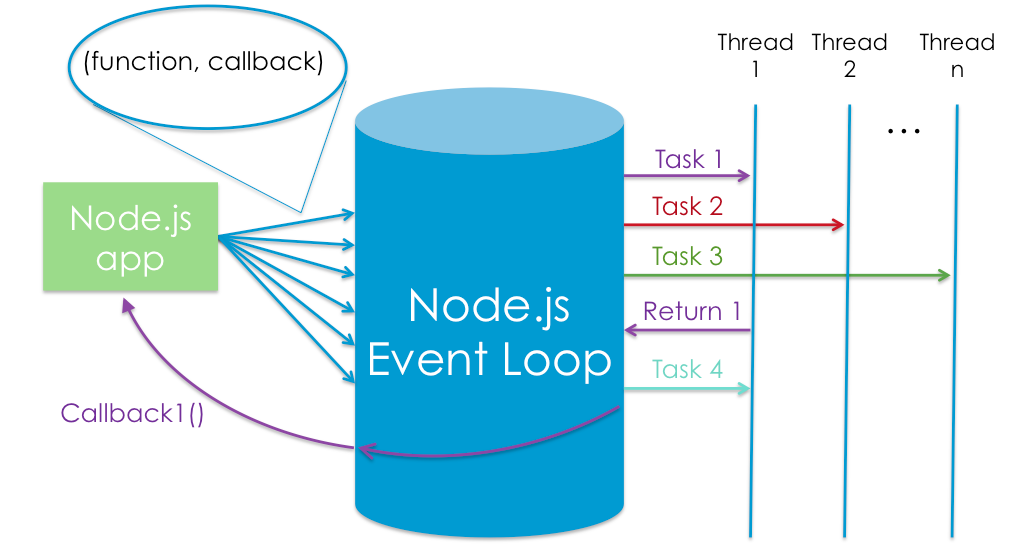
\includegraphics[width=\textwidth,height=\textheight,keepaspectratio]{eventLoop.png} 
\caption{Pętla zdarzeń w środowisku Node.js - źródło: http://galaxy.agh.edu.pl}
\end{figure}

\section{Asynchroniczność}
Node.js pracuje wykorzystując tylko jeden wątek używajac technologii asynchronicznego wejścia/wyjścia. 
Zapewnia to synchronizacje wykonywania wielu operacji bez konieczności czekania na zakończenie operacji i zwolnienie dostepu do zasobu poprzez zarządzanie żądaniami wejścia/wyjścia w oderwaniu od wątków wykonywania. 
Standardowe operacje synchroniczne powodują zablokowanie dalszego wykonywania wątku do czasu zakończenia przetwarzania. 
W rezultacie określony wątek może zainicjowac tylko jedno zadanie wejścia/wyjścia w jednym momencie. 
Wywołanie asynchroniczej funkcji nie czeka na wyniki, dzięki czemu nie blokujemy wątku wykonawczego. 
Po zakończonym wywołaniu uruchomiona zostaje funkcja zwrotna lub ogłoszone zostaje zdarzenie w poszczególnych częściach wykonawczych. 
Pomimo, że Node.js działa na jednym wątku z pętlą zdarzeń, dzięki asynchroniczności potrafi on obsłużyć więcej zapytań niż np. serwer HTTP Apache. 
Uzyskanie wielowątkowości pomimo korzystania tylko z jednego wątku jest zapewnione dzięki użyciu wzorca projektowego obserwator, w którym jeden obiekt nazywany przedmiotem obserwowanym określa zależności wzgledem obserwujących go innych obiektów, poprzez wywoływanie ich metod dla określonych własnych stanów. 
W celu obsługi wszystkich asynchronicznych funkcji oraz wątku głównego Node.js korzysta z biblioteki multiplatformowej języka c - libuv. 
Biblioteka ta została stworzona specjalnie na potrzebny Node.js, ale jest również wykorzystywana w wielu innych technologiach np racer: (obsługa serwerów w języku ruby), czy Trevi: (silnik do obsługi aplikacji internetowych w języku swift). 
Wykorzystuje ona określony zbiór wątków do równoległej obsługi wielu operacji wejścia/wyjścia bez wzajemnego ich blokowania. 
Wadą pracy Node.js przy wykorzystaniu tylko jednego wątku jest brak skalowalności pod względem możliwości zwiększenia ilości rdzeni procesorów, na których wykonuje sie program, bez użycia dodatkowych modułów takich jak Cluster (zapewnia możliwość łatwego tworzenia pochodnych procesów, które współdzielą porty serwera), StrongLoop PM (zapewnia zarządzanie procesem produkcyjnym aplikacji Node.js ze wsparciem odpowiedniego zarzadzania zasobami, wdrożeniami wielo hostowymi oraz interfejsem graficznym), czy PM2 (zarządzanie procesem produkcyjym, ze wsparciem odpowiedniego zarządzania zasobów z możliwością nieprzerwanego działania aplikacji przy użyciu przenoszenia jej między domenami bez potrzeby zatrzymywania pracy). 
Kolejną możliwością na uniknięcie tego ograniczenia jest zmiana ilości wątków należących do zbioru wykorzystywanego przez biblioteke libuv. 
Wątki te działają na wielu rdzeniach systemu na którym działa serwer. 
Działanie Node.js jednocześnie na wielu procesach jest zapewnione własnie dzięki zbiorowi wątków dostarczanych przez biblioteke libuv.
Wątek główny przydziela zadania dla wątków kolejno ze współdzielonej kolejki funkcji, które wątki pochodne maja za zadanie wykonać. 
Kiedy watek pochodny zakończy wykonywanie przydzielonego mu zadania informauje o tym wątek główny poprzez wywołanie określonego wywołania zwrotnego. 
Z przyczyny odpowiedzialności przez watek główny do odebrania wszystkich wywołań zwrotnych, funkcja wykonywana przez jeden wątek pochodny moze wstrzymać działanie całej asynchroniczenej opreracji, a co za tym idzie zmniejszyć jej całkowitą wydajność. 
Biblioteka libuv zajmuję się odpowiednim podziałem zadań oraz przydzieleniem zasobów tak aby w jak najlepszy sposób wyważyc nakład pracy między wieloma wątkami. 

\begin{figure}[!hb]
\centering
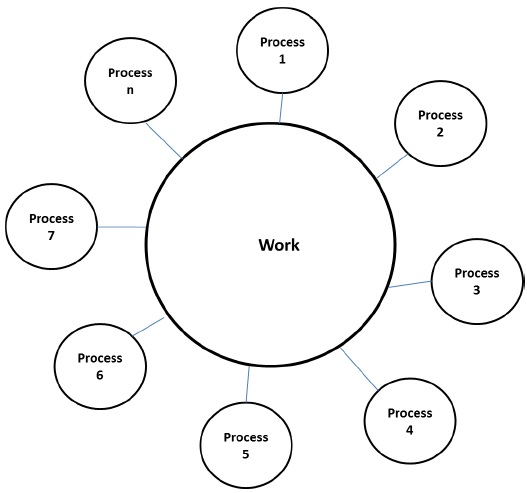
\includegraphics[width=\textwidth,height=\textheight,keepaspectratio]{thread.png} 
\caption{Model programowania współbieżnego wykorzystywany przez Node.js - źródło: www.tutorialspoint.com/parallel\_algorithm/}
\end{figure}

\section{Architektura komunikacji}
W tradycyjnym podejściu odpowiedzialne za obsługe przychodzących połączeń są określone wątki lub procesy sytemu operacyjnego, które w porównaniu z technologią Node.js wymagają względnie więcej zaalokowanych zasobów. 
W celu obsługi zapytania przychodzącego do aplikacji Node.js, program rejerstruje się w systemie operacyjnym, aby od każdego przychodzącego połączenia otrzymać odpowiednie wywołanie zwrotene, przez co nie potrzebuje procesów czy wątków aby uzyskać możliwość obsługi klientów, a tylko własnej pętli głównej, do której wykonywania powraca po przetworzeniu każdego wywołania wstecznego. 
W czasie pracy każde przychodzące połączenie otrzymuje odpowiednią ilość zasobów na stercie programu, więc nie ma rownież potrzeby alokowania zasobów dla każdego z wątków czy procesów osobno. 
Najbardziej popularna metoda na zarządzanie komunikacją między instancjami korzystajacymi z serwera używającego technologji Node.js jest wykorzystanie frameworku Restful Api popularnie zwanego Rest. 
Jest to wzorzec architektury oprogramowania, który opisuje sposób operowania zapytaniami pomiedzy Api, w prosty sposób poprzez obsługe zadań oraz odpowiedzi. 
Został on następnikiem protokołu sieciowego SOAP (Simple object Access protocol), stając się wiodącym standardem. 
Pozwala on na elimincaje zbędnej pracy i czasu wymaganego na integracje. 
Daje możliwość na stworzenie komunikacji bez potrzeby wiedzy na temat instacncji korzystajacych z przesyłanych zasobów - może integrować środowiska napisane w różnych językach działające na różnych platformach. 
Wykorzystuje proste zapytania przy użyciu protokolu http, oraz jego popularnie stosowanych metody takich jak post, get, put, delete oraz bardziej złożonych i używanych żadziej jak options, head, trace oraz connect. 
Opis typu zasobów jakie wymieniamy jest określony w nagłówku informacji przez kod statusu http. 
Poniższa tabelka prezęuje poszczególne typy statusów:

\begin{figure}[!hb]
\centering
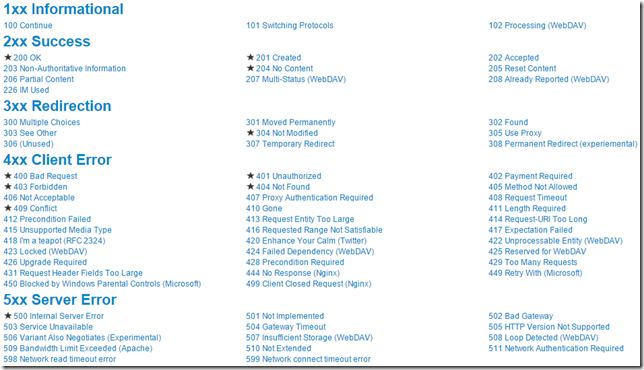
\includegraphics[width=\textwidth,height=\textheight,keepaspectratio]{statuses.png} 
\caption{Kody statusu protokołu http - źródło: http://mokandra.blogspot.fi/2015/10/http-status-code-definitions.html}
\end{figure}

W celu wymiany zasobów framework wykorzystuje najpopularniejsze sposoby opisu struktury służące do opisu obiektów takie jak najczęściej spotykany, najprostszy w użyciu format json (JavaScript Object Notation) oraz mniej popularny w technologi Rest format xml (eXtensible Markup Language). 
Różnica pomiędzy dwiema formami jest taka że xml jest językiem nie zdefiniowanych znaczników, a json tylko sposobem na prezęnacje właściwości obiektu. 
Porównanie obydwu struktur:
Struktura w formacie json opisująca listę pracowników:
\begin{lstlisting}[language=json,firstnumber=1]
{"employees":[
	{ "firstName":"James", "lastName":"Bond" },
	{ "firstName":"David", "lastName":"Klint" },
	{ "firstName":"Peter", "lastName":"Blom" }
]}
\end{lstlisting}

Ta sama struktura opisana w formacie xml:
<employees>
\begin{lstlisting}[language=XML,firstnumber=1]
	<employee>
		<firstName>James</firstName> <lastName>Bond</lastName>
	</employee>
	<employee>
		<firstName>David</firstName> <lastName>Klint</lastName>
	</employee>
	<employee>
		<firstName>Peter</firstName> <lastName>Blom</lastName>
	</employee>
</employees>
\end{lstlisting}


\chapter{Założenia i specyfikacja aplikacji}

\section{Specyfikacja problemu}
Potrzebny jest nowoczesny system do zarządzania tablicami zadań, który będzie posiadał autoryzowany dostęp dla użytkowników systemu. 
Został zauważony problem braku prostej w obsłudzę, intuicyjnej aplikacji pozwalającej we współpracy z innymi użytkownikami na zarządzanie zarówno podziałem jak i procesem realizacji wyszczególnionych zadań.
W celu reakcji na zapotrzebowanie zostanie zaprojektowany system informatyczny pracujący w technologii Node.js, ze względu na możliwą do osiągniecia niezawodność oraz dostępność nawet przy jednoczesnej obsłudze wielu korzystających z aplikacji klientów.
Nie powinien on wymagać żadnych procesów wdrożeniowych w celu zrozumienia obsługi narzędzia, ponieważ celem projektu jest stworzenie narzędzia, które wspiera, a nie dodatkowo komplikuje określone zadania.
System powinien w przejrzysty sposób prezęować proces realizacji poszczególnych zadań zorganizowanych w tablicach.
Właściel określonej tablicy powinien mieć możliwość zarządzania dostępem do tablicy poprzez udostępnianie lub ograniczanie jej treści pozostałym użytkowniką.
Aplikacja zapewni subskrybentą nieprzerwaną możliwość nadzoru, wglądu oraz określania aktualnych statusów dowolnych procesów.

\section{Wymagania funkcjonalne}
Analiza wymagań funkcjonalnych umożliwia zidentyfikowanie i opisanie pożądanego zachowania systemu. 
Umożliwiają określenie usług oferowanych przez system, reakcji na dane wejściowe oraz zachowania w określonych sytuacjach.
\begin{itemize}
\item Wymiana komunikatów w modelu klient-serwer.
\item Możliwość utworzenia do 1000000 kont użytkowników.
\item Możliwość zmiany danych użytkownika.
\item Weryfikacja adresu email przez aktywacją.
\item Możliwość resetowania hasła za pomocą adresu email.
\item Utrzymanie do 100 tablic jednocześnie dla użytkownika.
\item Możliwość usuwania tablic.
\item Obsługa do 1000 równoległych członków jednej tablicy.
\item Możliwość zarządzania członkami tablicy.
\item Obsługa do 10000 równoległych zadań dla tablicy.
\item Możliwość usuwania zakończonych zadań.
\item Utrzymanie do 1000 statusów do jednego zadania.
\item Zapamiętywanie terminu zmiany statusu zadań.
\item Walidacja poprawności wprowadzanych przez użytkownika danych zarówno po stronie klienta jak i serwera.
\item W razie wystąpienia nieprawidłowych danych system powiadamia o błędach.
\item Zapewnienie okna pomocy opisującego korzystanie z aplikacji.
\item Możliwość otrzymywania powiadomień o aktualnym statusie tablic oraz poszczególnych zadań.
\item System współpracuje z bazą danych.
\end{itemize}

\section{Wymagania pozafunkcjonalne}
Wymagania niefunkcjonalne opisują kryteria umożliwiające możliwość oceny działania systemu i elementów mających wpływ na satysfakcję użytkownika.
Zdefiniowane zostały następujące wymagania niefunkcjonalne:

\begin{itemize}
\item Dostęp do określonych zasobów musi być chroniony poprzez login i hasło użytkownika.
\item Budowa interfejsu użytkownika musi być możliwie intuicyjna i prosta w obsłudzę.
\item Proste analizowanie i diagnozowanie błędów oraz sytuacji problemowych.
\item Budowa zapewnia łatwe wprowadzanie koniecznych zmian.
\item Jest w stanie obsłużyć jednocześnie do 100.000 użytkowników.
\item Czas uruchomienia jest nie dłuży niż 10 sekund.
\item Umożliwia efektywne testowanie wprowadzonych zmianach.
\item Możliwość obsługi poprzez różne przeglądarki internetowe i środowiska.
\item Zrozumiały dla wszystkich. Czas przyswojenia nie przekracza 15 minut.
\item Ma możliwość współistnienia z innymi modułami.
\item Spełnia wszystkie normy prawne w naszym kraju.
\end{itemize}

\chapter{Opracowanie aplikacji}

\section{Mean Stack}

\subsection{Wstęp}
Do opracowania rozwiązania zdecydowałem się skorzystać z Mean Stack. 
Skrót odnosi się do frameworków oraz technolgji Mongodb, Express, AngularJS oraz Node.js. 
Współpracując razem zapewniają bardzo szybkie efektywne tworzenie skalowalnych aplikacji wielopratformowych. 
Do użycia wszystkich wymagany jest tylko jeden język programowania - javaScript, zarówno do obsługi warstwy frontend'owej aplikacji jak i backend'owej. 
Wszystkie technolgie są dostępne w pełni bezpłatnie. 
\begin{figure}[!hb]
\centering
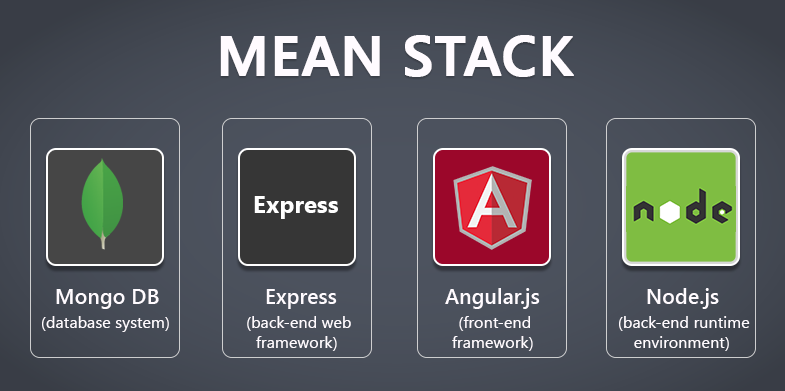
\includegraphics[width=\textwidth,height=\textheight,keepaspectratio]{meanStack.png} 
\caption{Przedstawienie technologii MEAN Stack - źródło: http://codecondo.com/7-good-reasons-to-use-mean-stack-in-your-next-web-project/}
\end{figure}

Technologia Node.js została już opisana powyżej, więc zajmę się opisem pozostałych.

\subsection{MongoDB}
Napisany w języku c++ system zarządzania bazą danych zorietowanym na dokumenty. 
Operuje na nierelacyjnych bazach danych. 
Używa struktur json jako schematów budowy bazy danych.
Udostepnia całkowitą dowolność w budowie struktury wymaganej bazy danych. 
Wykorzystuje proste, ale zapewniające szerokie możliwości zapytania bazo danowe.

\subsection{ExpressJS }
Framework slużący do szybkiego wymagającego jak najmniejszych nakładów pracy wytwarzania zarówno backend’u aplikacji internetowych jak i aplikacji mobilnych.
Dostarcza zbiór określonych klass i metod. Jest to najpopularniejszy framework do tworzenia serwerów w technologi Node.js.

\subsection{AngularJS}
Wykorzystujący wzorzec projektowy MVC (Model View Controler) polegający na oddzieleniu od siebie poszczegolnych warstw aplikacji - logiki, widoku oraz modelu komunikacji, framework wykorzystujacy dodatkowe tagi w języku html w celu prostego w obsłudze i nie wymagającego dodatkowej logiki napisanej w języku javaScript tworzenia dynamicznych stron internetowych.

\section{Komunikacja}

\subsection{Rozwiązanie problemu komunikacji}
Do komunikacji między warstą frontend'ową i backendow'ową po stronie klienta wykorzystałem wysokopoziomową biblioteke Ajax oraz technologie Restful api. 
Ajax polega na zarządzaniu asynchroniczna komunikacja. 
Dzięki temu aplikacjia może wykonywać inne funkcje mimo oczekiwania na odpowiedź ze strony serwera, za sprawa odseparowania warstwy wymiany danych od pozostałych warstw aplikacji.
Do opisu wymienianych struktur użyłem standardu json, ponieważ wymaga on mniejszych nakładów pracy od standradu xml. 
Powyższe frameworki współpracują ze sobą w bardzo intuicyjny i przejrzysty sposób. 
Angular prezętuje dynamiczną aplikacje internetowa użytkownikowi, odpowiada za przyjmowanie danych i z pomoca ajax'a wysyła oraz odbiera dane wysyłane do serwera. 
Serwer Node.js z użyciem technologii express wykorzystując metode routingu dopasowuje zapytanie do odpowiednich funkcji serwisu, przetwarza otrzymane dane, przy współpracy z bazą danych zarządzana przez Mongodb przechowuje informacje użytkowników serwisu oraz w odpowiedzi zwraca odpowiednie dane spowrotem do warsty frontendowej prezęującej dane użytkownikowi. 

\begin{figure}[!hb]
\centering
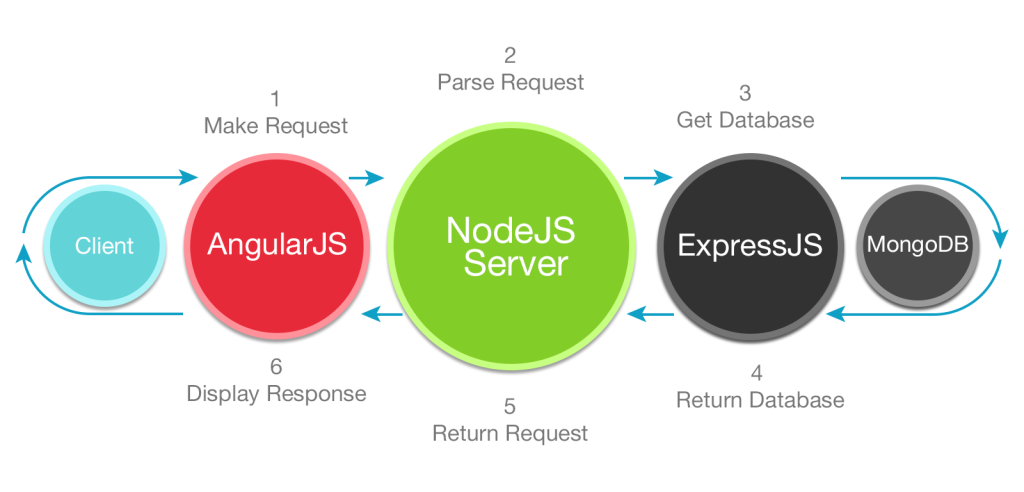
\includegraphics[width=\textwidth,height=\textheight,keepaspectratio]{Meanex.png}
\caption{Przepływ komunikacji w MEAN Stack źródło: https://www.dealfuel.com/seller/mean-stack-tutorial/}
\end{figure}

\subsection{Schematy wymiany zasobów}
Uniwersalny dla aplikacji schemat procesu pobrania statycznych zasobów z serwera wykorzystuje metode get. Do zasobów tych należy miedzy innymi plik html zawierający warstwe prezęacji aplikacji, plik css zawierający styl warstwy prezętacji czy plik zawierający funkcje wykorzystywane przez aplikacje w języku javaScript. Proces prezęnuje sie nastepujaco:
\begin{figure}[!hb]
\centering
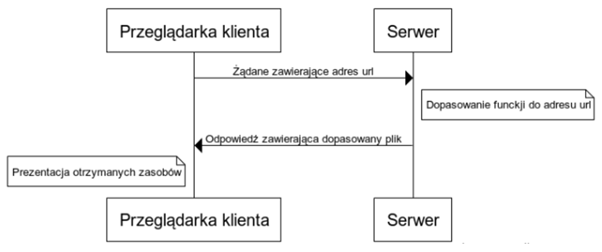
\includegraphics[width=\textwidth,height=\textheight,keepaspectratio]{K-S.png} 
\caption{Pobranie statycznych zasobow źródlo: Opracowanie własne}
\end{figure}
\begin{enumerate}
\item Klient przy użyciu przeglądarki wysyła pod określony adres url serwera zapytanie zawierające porządany zasób.
\item Serwer otrzymuje zapytanie i dopasowuje określoną funkcje po adresie url serwera.
\item Funkcja wybiera dopasowane do zapytania zasoby i wysyła odpowiedź do aplikacji.
\item Aplikacja odbiera i zaczyna korzystac z zasobów.
\end{enumerate}

 Uniwersalny dla aplikacji schemat procesu wymiany danych określonych dla specyficznego użytkownika wykorzystuje metode post. Przykładowe dane wymieniane przez aplikacje to login, hasło, informacje odnośnie żądań użytkownika, komętarze do zadań użytkownika. Przepływ danych wygląda następująco:
 \begin{figure}[!hb]
\centering
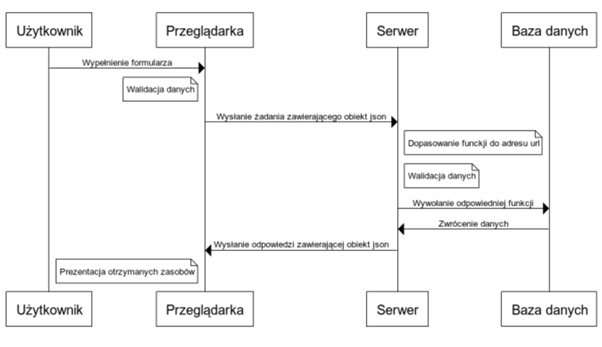
\includegraphics[width=\textwidth,height=\textheight,keepaspectratio]{U-P-S-B.png} 
\caption{Wymiana zasobów w formacie Json źródlo: Opracowanie własne}
\end{figure}
\begin{enumerate}
\item Dane zostaja pobrane od użytkownika w określonym formularzu w warstiwe frontendowej.
\item Dane zostają zwalidowane pod kątem poprawności po stronie użytkownika.
\item Jesli dane są poprawne zostaja zorganizowane w obiekcie json i wysłane do serwera, w przeciwnym wypadku zostaje zwrócony błąd.
\item Serwer odbiera zapytanie i przekazuje je do odpowiedniej funkcji.
\item Dane zostają zwalidowane pod kątem poprawności po stronie serwera.
\item Jeśli dane są poprawne serwer realizuje określona funkcje przy pomocy zapytań bazo danowych, w przeciwnym wypadku zostaje przygotowany komunikat o błędzie.
\item Odpowiedź na zapytanie bazodanowe zostaje odebrane i zostają przygotowane dane do wysłania.
\item Przygotowane dane zostaje wysłane w określonej odpowiedzi.
\item Warstwa frontendowa otrzymuje odpowiedź i zostaje odświeżona warsta prezętacji aplikacji.
\end{enumerate}
 

\subsection{Kod po stronie klienta wysyłający żądanie}
Przykładowy kod wykonywany po stronie klienta wysyłający żądanie do serwera, żadające określonego zasobu przy użyciu frameworku Angularjs:
Plik w języku javaScript zawierający definicje modelu i kontrolera:
\medskip
\begin{lstlisting}
var main = angular.module("main", []); 									// create angular module

main.controller('SignInController', function($scope) { 					// create controller for module
	$scope.login=""; 													// initialize login as field in model
	$scope.password=""; 												// initialize password as field in model
	$scope.SignIn=function(){ 											// callback function as field in model
		if ($scope.login && $scope.password) {							// if both field are filled
			var xhr = new XMLHttpRequest();									//create request object
			xhr.open("POST", http://site.com/authorization, true);		// set method type, domain address and is it asynchronous
			xhr.setRequestHeader("Content-type","application/json");	// set header with information of content type
			req.send(JSON.stringify({	login: $scope.login,			
										password: $scope.password})); 	// Send json object with login and password
			req.onreadystatechange = function() { 						// create callback, called on every state change
				if (req.readyState === 4) { 							// readyState 4 is 4 when respond is got
					if (req.status === 200) { 							// http status code 200 - ok
						var resObj = JSON.parse(this.responseText);		// parse response text to json object
						$scope.login=resObj.login;						// set password from response
						$scope.password=$resObj.password;				// set password from response
						alert("Login and password are valid");			// alert user
					}
					else if (req.status === 401){						// http status code 200 -  Unauthorized
						$scope.invalid=req.responseText;  				// set response message containing error in view model
						$scope.$apply(); 								// apply changes on view model
					}
					else{ 												// all other http statusses
						alert(req.status+":"req.responseText); // alert user
					}
				}
			}
		}
	}
}
\end{lstlisting}

Plik w języku html zawierający definicje widoku:
\begin{lstlisting}[language=HTML]
<!DOCTYPE html> 
<!-- Apply view to model -->
<body ng-app = "main">
	<!-- Create form for request -->
	<form class="main" name="form""> 
		<table>
			<tr>
				<td style="width:50%;">
					Login
				</td>
				<td style="width:50%">
						<!-- Get user login -->
						<input type = "text" ng-model = "login" name="login"
							<!-- Set field validation -->
							required ng-pattern='/^[a-zA-Z0-9._-]+$/'  ng-maxlength="20" ng-minlength="3">
				</td>
			</tr>
			<tr>
				<td style="width:50%;">
					Password
				</td>
				<td style="width:50%">
						<!-- Get user password -->
						<input type = "text" ng-model = "password" name="password"
						<!-- Set field validation -->
							required ng-pattern='/^[a-zA-Z0-9._-]+$/'  ng-maxlength="20" ng-minlength="3">
				</td>
			</tr>
			<tr>
				<td colspan="2">
					<!-- show error message field from server only if invalid field exist -->
					<p ng-show="invalid">{{invalid}}</p>
					<!-- show static error message only if one of user field are invalid -->
					<p ng-show="form.login.$invalid || form.password.$invalid">Invalid login or password</p>
				</td>	
			</tr>
		</table>
	</form>
</body>
\end{lstlisting}

\subsection{Kod po stronie serwera obsługujący odebranie żądania}
Przykładowy kod wykonywany po stronie serwera obsługujący odebrane żądanie od klienta przy użyciu technologii Node.js oraz framework'ów express i mongodb:
\medskip
\begin{lstlisting}
var express = require('express');					// load express module
var bodyParser = require('body-parser');    		// load module for parsing json data
var dataBase = require('mongodb').MongoClient;  	// load MongoDB database module
var Promise = require('promise');               	// load asynchronous returns from functions module
var dataBaseUrl = "mongodb://localhost:27017/db"; 	// dataBase address

var port = 8081;  									// application port
var app = express();						        // create epress configuration object
app.use(bodyParser.json());                         // load bodyParser to app object
app.use(bodyParser.urlencoded({ extended: true })); // for parsing application/x-www-form-urlencoded

// connect to database function, returns database handler
function Connect() {
    return new Promise(function (fulfill, reject) {
        dataBase.connect(dataBaseUrl, function(err, db) {
            if (err) {
                reject(err);
            }
            fulfill(db);
        });
    });
}

// check if database contains given user
var Authorization=function (login, password) {
    return new Promise(function (fulfill, reject) {
        Connect().done(function (db) {
            db.collection("Users").findOne({ login: login, password: password }, function (err, result) {
                if (err) {
                    reject(err);
                } else {
                    if (result != null) {
                        fulfill(true);
                    }
                    else {
                        fulfill(false);
                    }
                }
                db.close();
            });
        });
    });
}

// check is text format correct
function TextValidation(text, min, max) {
    if (min === undefined) min = 0;
    if (max === undefined) max = Infinity;
    return (text !== undefined) && (/^[a-zA-Z0-9._-]+$/).test(text) && text.length >= min && text.length <= max;
}

// check is user credentials data correct
function UserValidation(body) {
    return new Promise(function(fulfill, reject) {
        if (!TextValidation(body.login, 3, 20) || !TextValidation(body.password, 3, 20)) {
            fulfill(false);
            return;
        }
        Authorization(body.login, body.password).done(function (authentication) {
            fulfill(authentication);
        });
    });
}

//funtion run when server gets post request with url /authorization
app.post('/authorization', function (req, res) {
	UserValidation(req.body).done(function(valid) {
	    if (valid) {
	  	    res.setHeader('Content-Type', "text/html");
			res.statusCode = 200;
			res.end();
	   	}
        else {
            res.setHeader('Content-Type', "text/html");
			res.statusCode = 401; // error has happend
			res.write("Invalid login or password");
			res.end();
		}
    });
});

//start server
var server = app.listen(port, function () {
	MakeLog('Server listening');
});
\end{lstlisting}

\section{Wykorzystane moduły}

\subsection{Moduły zewnętrzne}
Zewnętrzne moduły, zainstalowane za pomocą zbioru repozytorium npm, które użyłem do realizacji rozwiazania to:
\begin{enumerate}
\item express - opisany powyżej
\item fs - file stream, odpowiada za obsługe zapisu oraz wczytywania plików. 
Wykorzystywany w celu wczytywania plików statycznych aplikacji takich jak index.htm (strona główna w formacie html), main.js (funkcje w języku javaScript), style.css (plik arkuszu stylów, odpowiadający za styl prezętacji), favicon (ikona serwisu wyświetlana w oknie przeglądarki), czy losowo wybieranych zdjęć wyświetlanych w tle serwisu.
\item path - obsługa różnic między systemami operacyjnymi. 
Dzięki temu modułowi możemy zapewnić całkowitą sprawność naszego serisu nie zależnie od środowiska uruchomieniowego. 
Pozwala niwelować różnice w lokalizacji plików systemowych, czy łącznikach pomiędzy poszczególnymi folderami przy specyfikacji scieżki do pliku.
\item body-parser - dostarcza możliwość analizowania danych załączonych do odebranego przez serwer żądania, wykorzystany został w celu odczytów poszczególnych wartości odebranych w formacie json.
\item promise - odpowiada za operowanie wynikami otrzymanymi w wyniku asynchronicznych funkcji. 
Dzięki temu modułowi nie musimy synchronicznie czekać na otrzymanie zwrotu z kolejnych funkcji, natomiast możemy przy użyciu wywołań zwortnych zareagować po otrzymaniu określonego wyjścia.
\item cookie-parser - zapewnia możliwość wykorzystania plików cookie dla specyficznego klienta. 
Dzięki temu modułowi możemy ustawiać, usuwać lub edytować wartości plików cookie, które zostaną przydzielone dla konkretnego użytkownika w ramach całej sesji komunikacji z użytkownikiem lub przez określony przez nas czas. 
\end{enumerate}

\subsection{Moduły wewnetrzne}
Wewnetrzne moduły, czyli takie które zostały napisane przeze mnie specjalnie na użytek projektu to:
\begin{enumerate}
\item emails.js (wykorzystujący zewnętrzny moduł mongodb) - moduł zapewnia komunikacje z baza danych w technologii mongodb, poprzez wywoływanie odpowiednich funkcji. 
Został dostosowany bezpośrednio do obsługi bazy danych dla wykonywanego projektu. 
Dzięki temu plik główny serwera nie musi znać budowy, ani wykonywać operacji bezpośrednio na dokumentach bazy danych.
\item db.js (wykorzystujący zewnętrzny moduł nodemailer) - dostarcza obsługę wysyłania wiadomości email do użytkowników serwisu w przypadku zajścia określonych sytułacji takich jak na przykład otrzymanie nowego zaproszenia czy zmiana statusu zadania. Moduł dostarcza jedną, prostą w obsłudze funkcje zapewniającą obsługe wiadomości emial. 
\end{enumerate}
 
\chapter{Testy aplikacji}

Po wykonaniu aplikacji zostały przeprowadzone testy manualne sprawdzające poprawność dostarczanej przez serwis funkcjonalności.
Kolejne przypadki testowe:

\section{Uzyskanie dostępu do statycznych zasobów serwisu}
\begin{figure}[!hb]
\centering
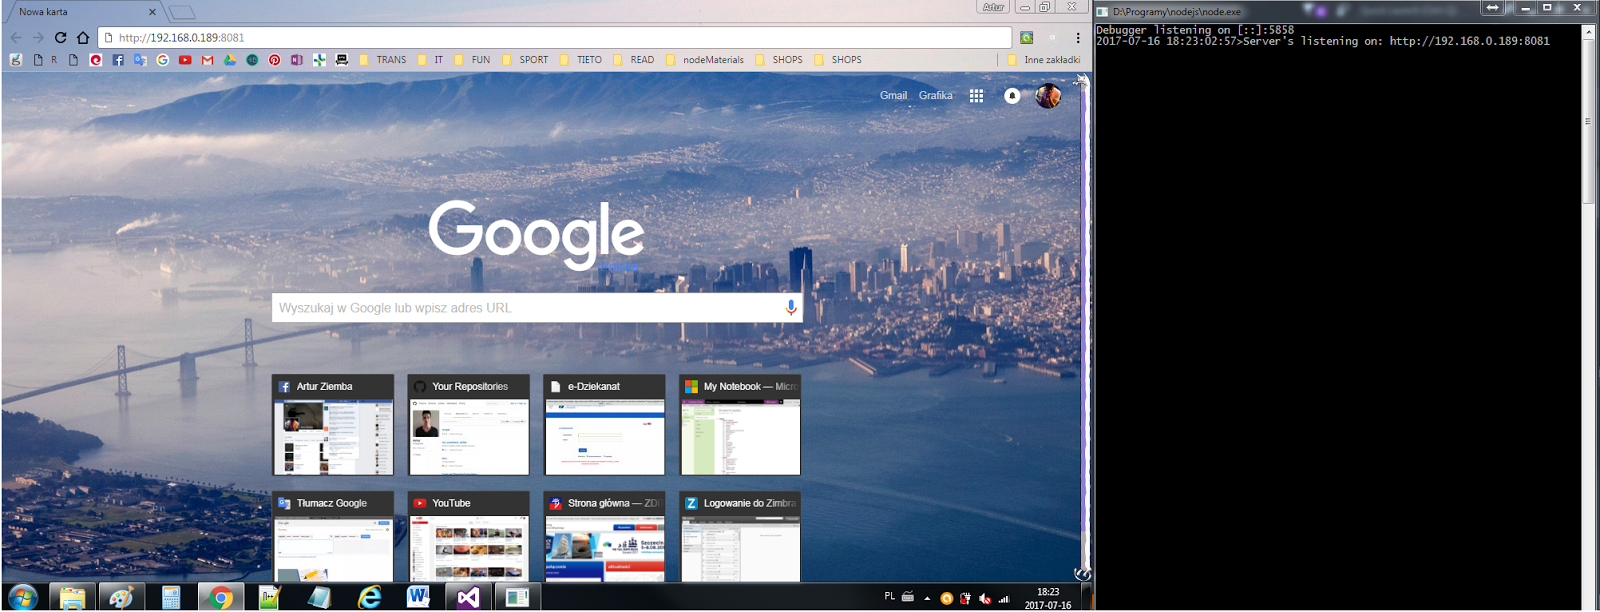
\includegraphics[width=\textwidth,height=\textheight,keepaspectratio]{11.png}
\captionsetup{labelformat=empty}
\caption[]{Użytkownik wysyła żądanie pod adres serwera.}
\end{figure}
\begin{figure}[!hb]
\centering
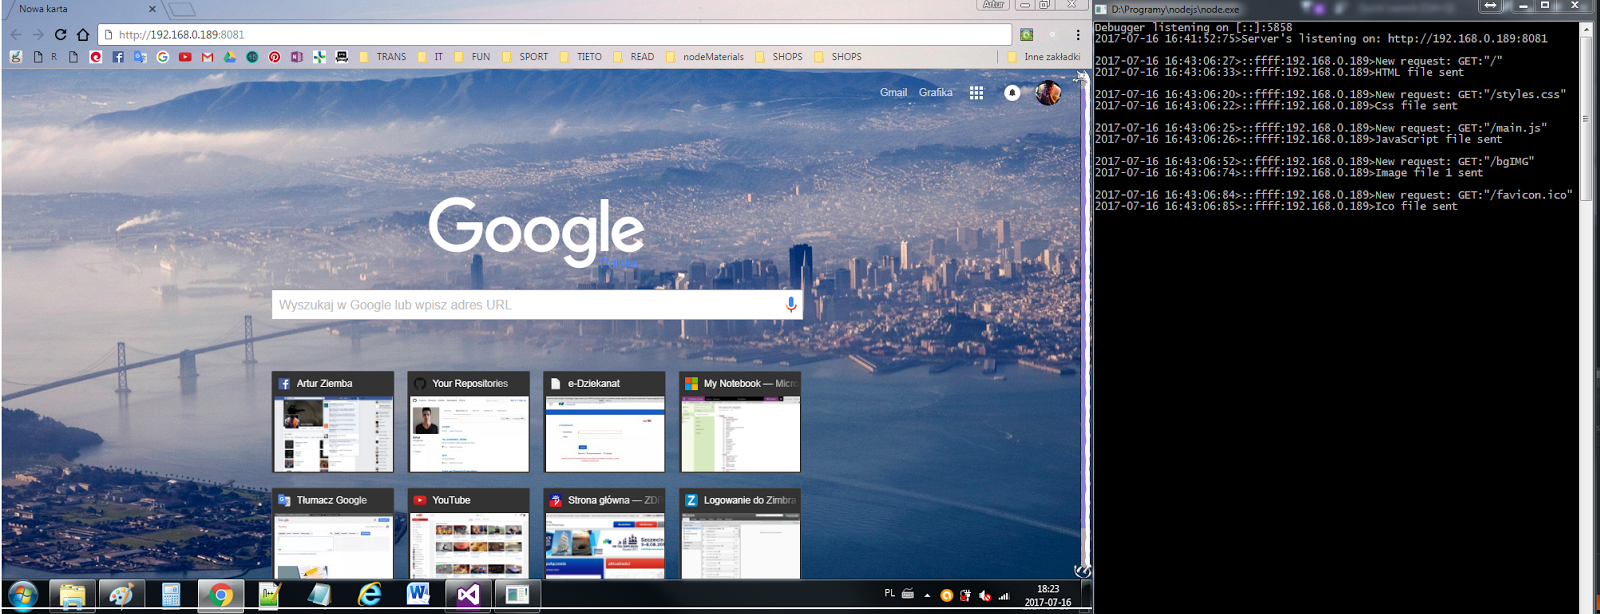
\includegraphics[width=\textwidth,height=\textheight,keepaspectratio]{12.png}
\captionsetup{labelformat=empty}
\caption[]{Użytkownik otrzymuje odpowiedź zawierająca pliki statyczne serwisu (plik html, css, js, zdjęcie w tle i favicon.}
\end{figure}

\section{Rejerstracja w serwisie}
\begin{figure}[!hb]
\centering
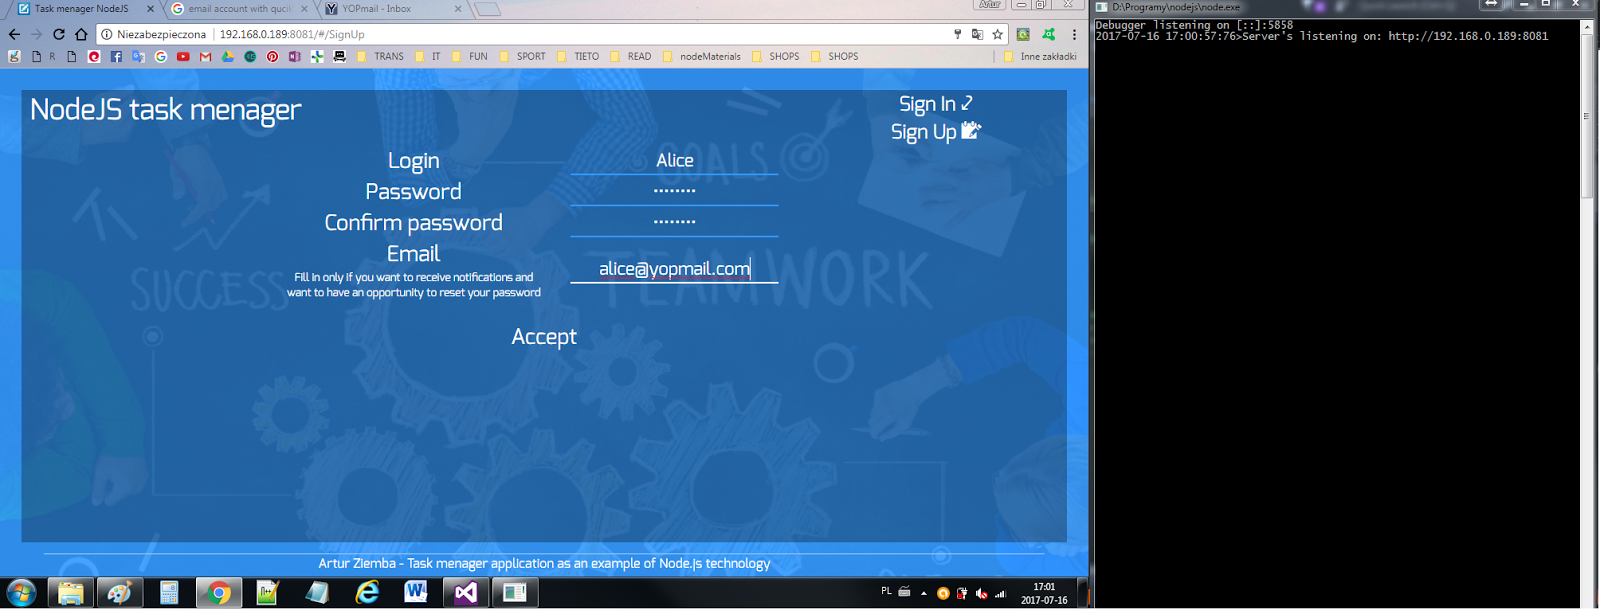
\includegraphics[width=\textwidth,height=\textheight,keepaspectratio]{21.png}
\captionsetup{labelformat=empty}
\caption[]{Użytkownik wypełnia formularz rejerstracyjny na stronie serwisu i wysyła dane do serwera. }
\end{figure}
\begin{figure}[!hb]
\centering
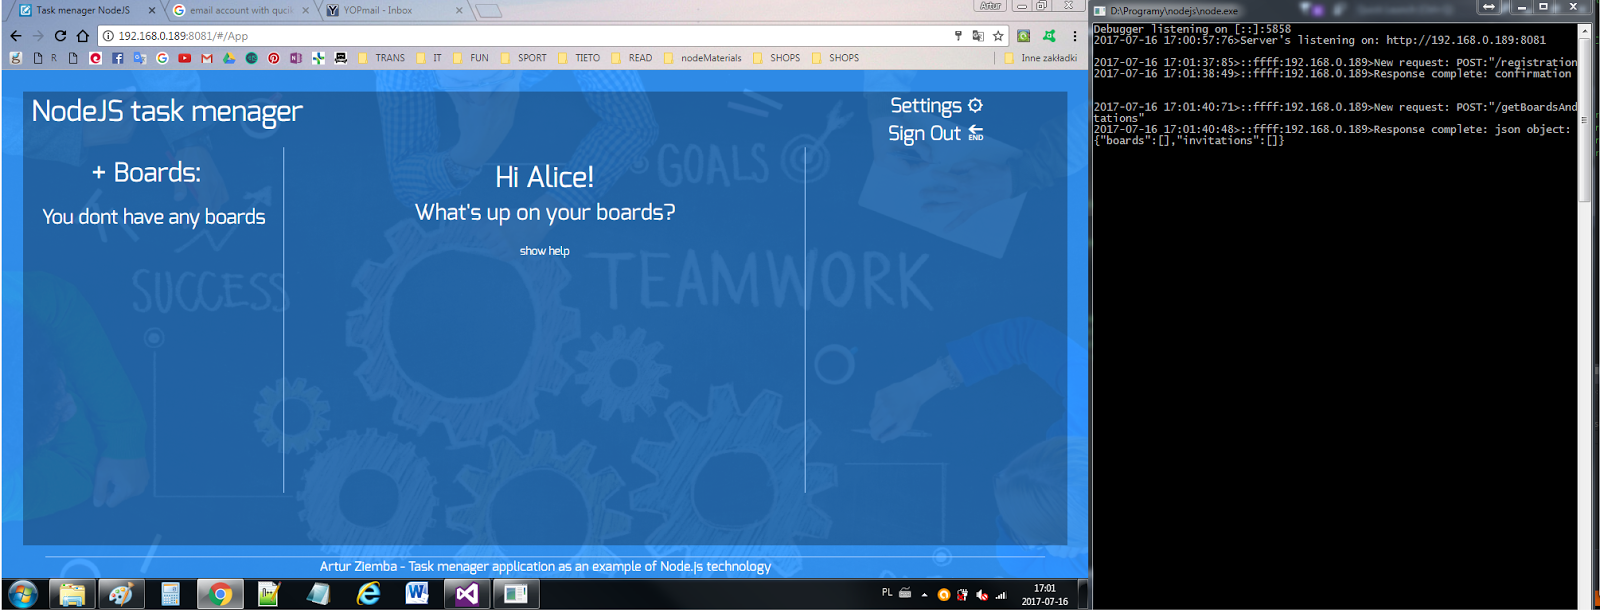
\includegraphics[width=\textwidth,height=\textheight,keepaspectratio]{22.png}
\captionsetup{labelformat=empty}
\caption[]{Serwer sprawdza poprawność otrzymanych danych i w odpowiedzi przesyła strone główną aplikacji dostępna po zalogowaniu na konto lub informacje o blędzie.}
\end{figure}


\section{Potwierdzenie adresu email}
\begin{figure}[!hb]
\centering
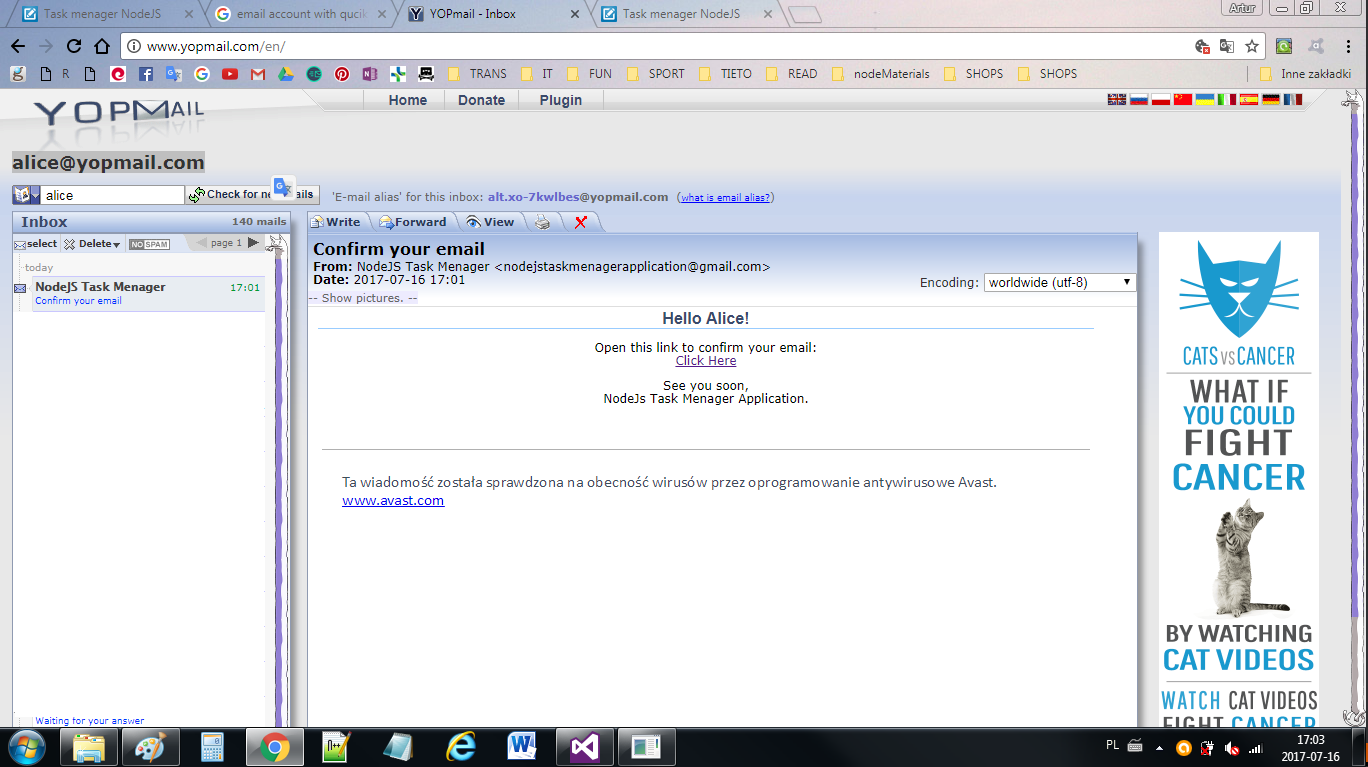
\includegraphics[width=\textwidth,height=\textheight,keepaspectratio]{31.png}
\captionsetup{labelformat=empty}
\caption[]{Po podaniu adresu email użytkowik otrzymuje wiadomość email zawierającą link aktywacyjny.}
\end{figure}
\begin{figure}[!hb]
\centering
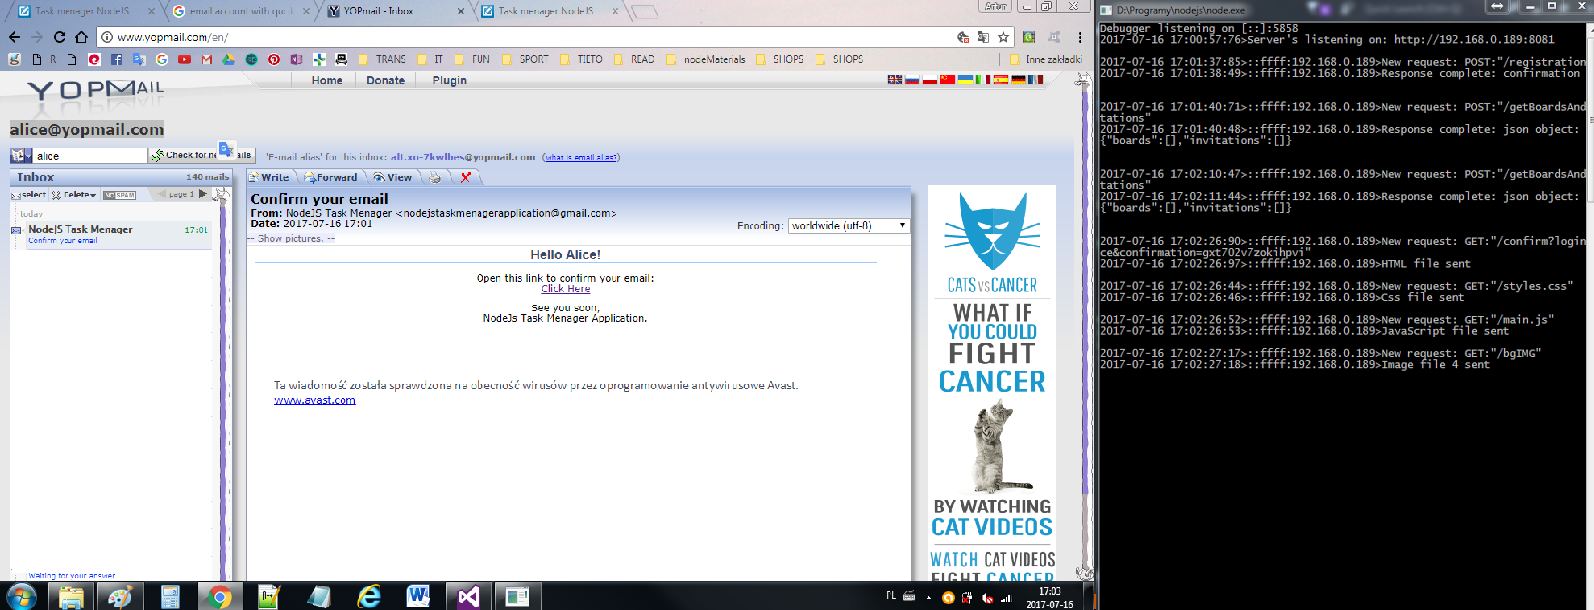
\includegraphics[width=\textwidth,height=\textheight,keepaspectratio]{32.png}
\captionsetup{labelformat=empty}
\caption[]{Po kliknieciu w link. Serwer sprawdza czy otrzymany w linku kod jest prawidłowy dla podanego użytkownika. 
Następnie aktywuje adres email dla odpowiedniego użytkownika i wysyła w odpowiedzi strone główną aplikacji oraz wiadomość email o potwierdzeniu.}
\end{figure}


\section{Logowanie się w serwisie}
\begin{figure}[!hb]
\centering
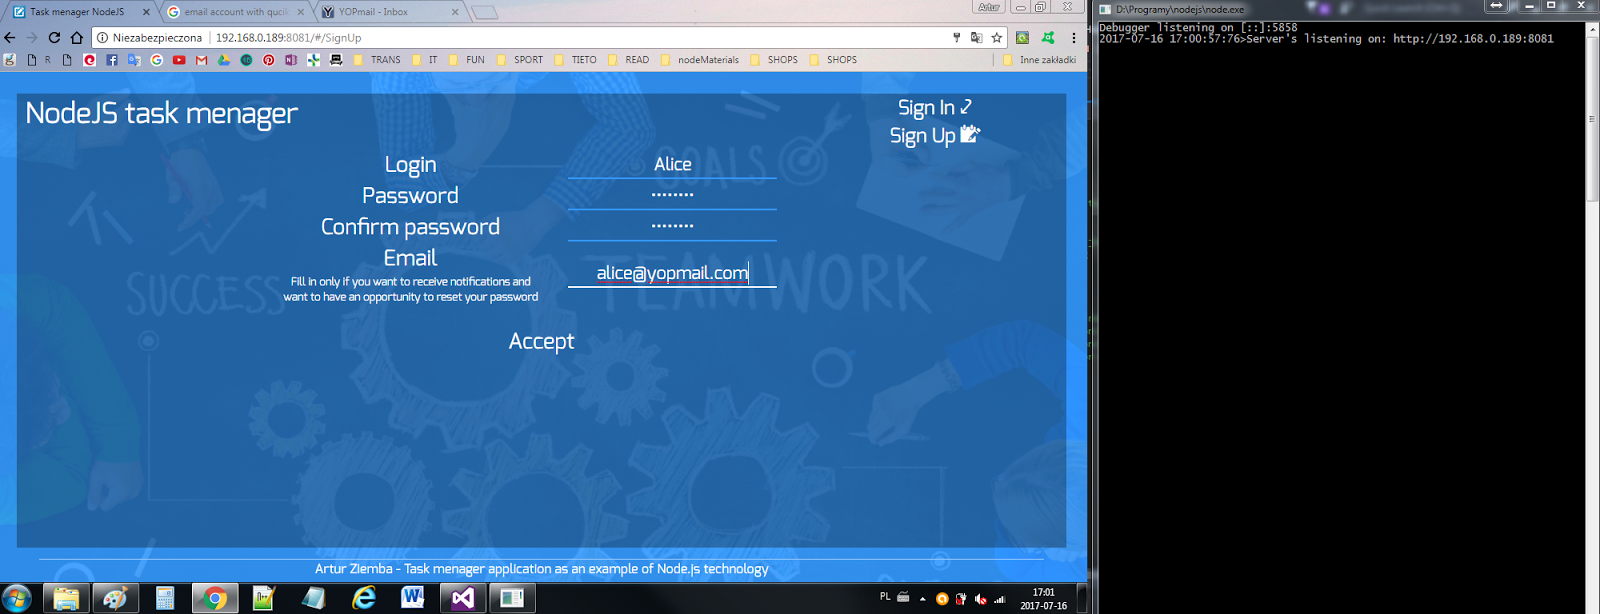
\includegraphics[width=\textwidth,height=\textheight,keepaspectratio]{41.png}
\captionsetup{labelformat=empty}
\caption[]{Użytkownik wypełnia formularz na stronie serwisu i przesyła żądanie do serwera.}
\end{figure}
\begin{figure}[!hb]
\centering
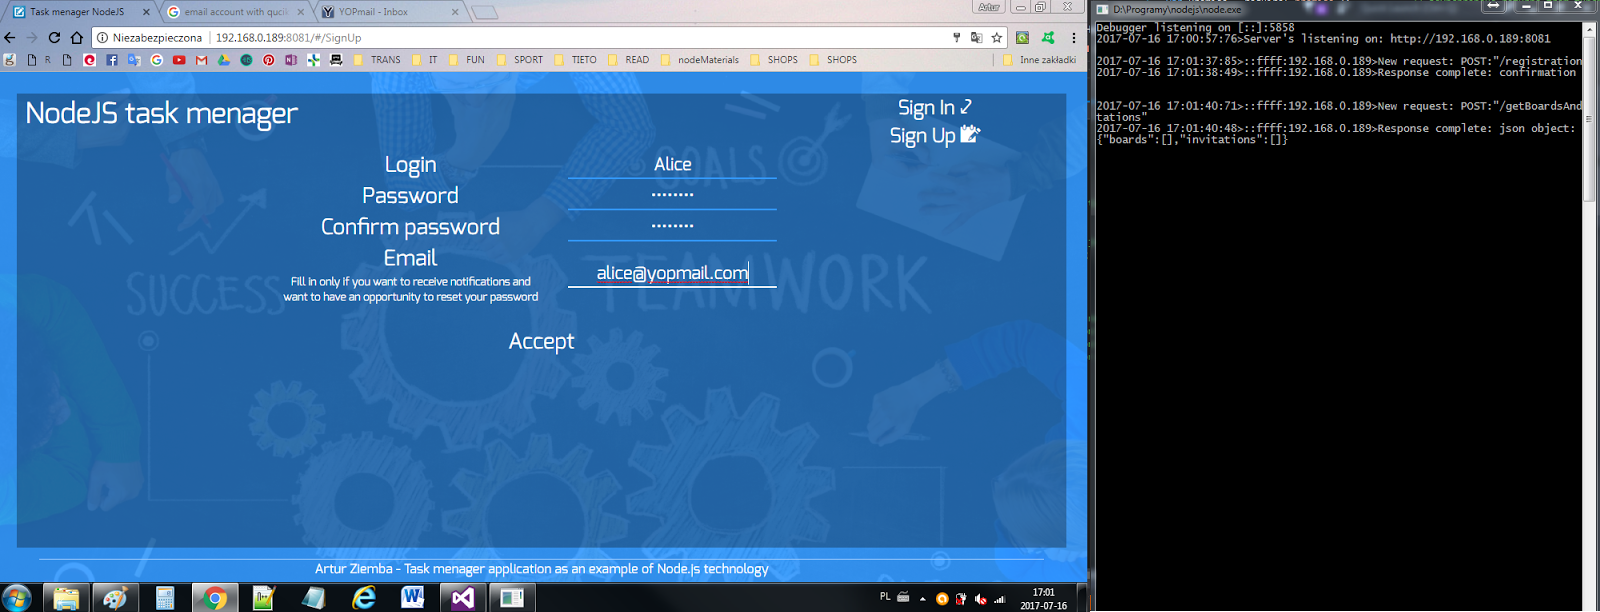
\includegraphics[width=\textwidth,height=\textheight,keepaspectratio]{42.png}
\captionsetup{labelformat=empty}
\caption[]{Serwer sprawdza istnienie konta w serwisie. 
W odpowiedzi użytkownik otrzymuje stronę główną aplikacji lub błąd o niepoprawnych danych.
W czasie bycia zalogowanym co określony czas zostaje wysłane żądanie aktualizacji danych. 
Aktualizacja następuje również każdorazowo po otrzymaniu pomyślnego potwierdzenia wykonania operacji przez serwer.}
\end{figure}


\section{Resetowanie hasła użytkownika}
\begin{figure}[!hb]
\centering
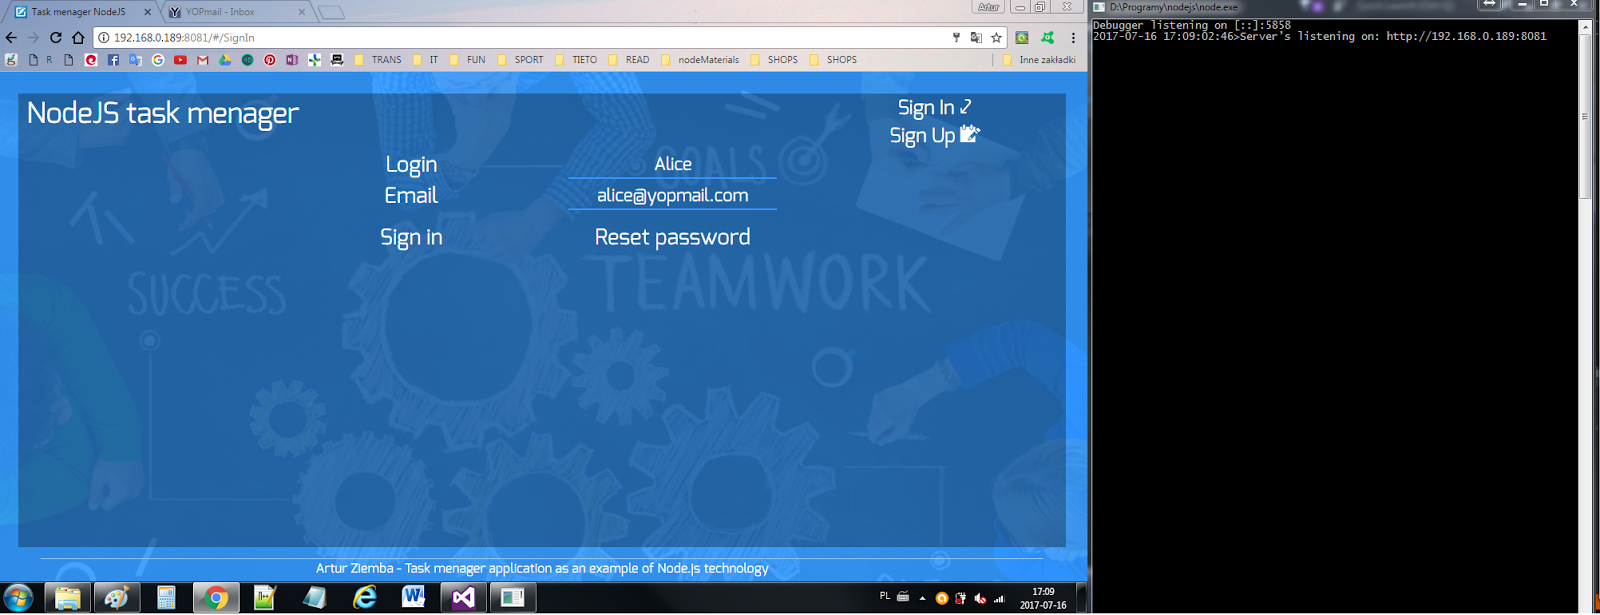
\includegraphics[width=\textwidth,height=\textheight,keepaspectratio]{51.png}
\captionsetup{labelformat=empty}
\caption[]{Funkcja jest dostępna po potwierdzeniu adresu email dla konta. 
Po wypełnieniu odpowiedniego formularza na stronie głównej serwisu użytkownik wysyła żądanie do serwera.}
\end{figure}
\begin{figure}[!hb]
\centering
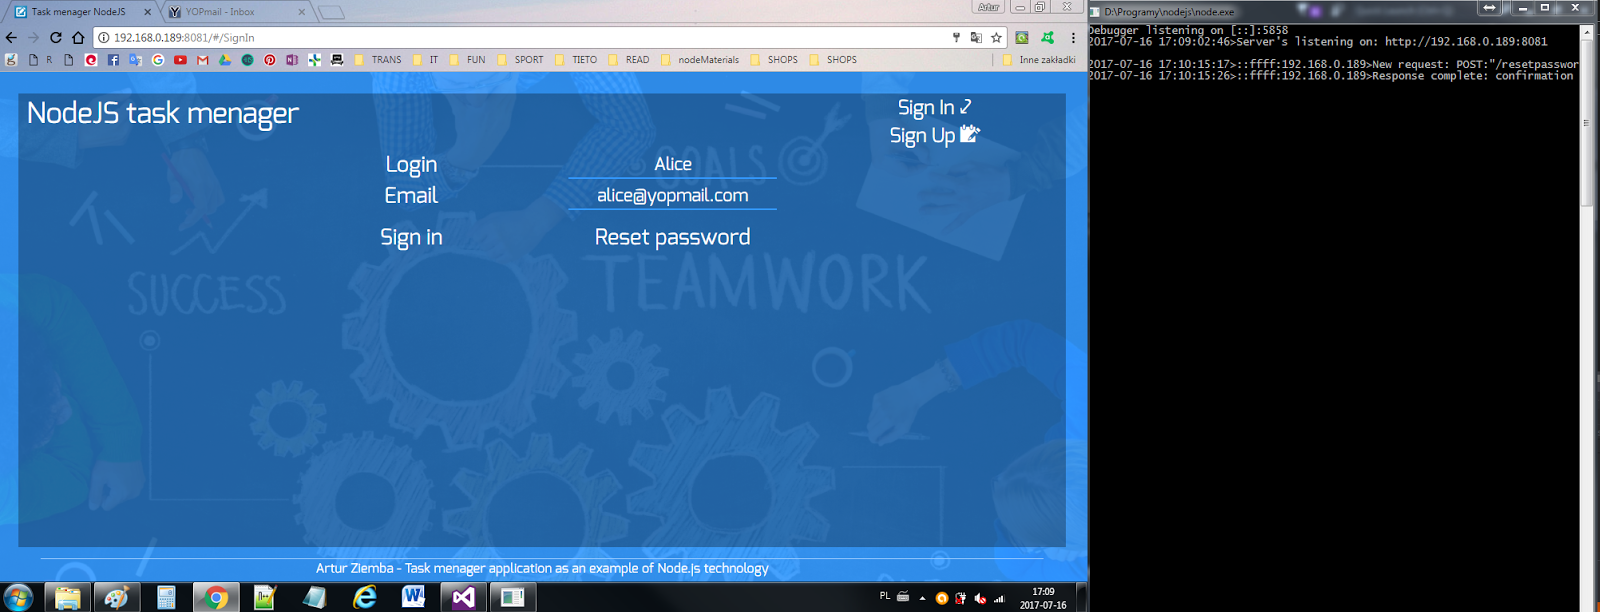
\includegraphics[width=\textwidth,height=\textheight,keepaspectratio]{52.png}
\captionsetup{labelformat=empty}
\caption[]{Serwer sprawdza podane dane. W odpowiedzi wysyła informacje o przetworzeniu żądania.}
\end{figure}
\begin{figure}[!hb]
\centering
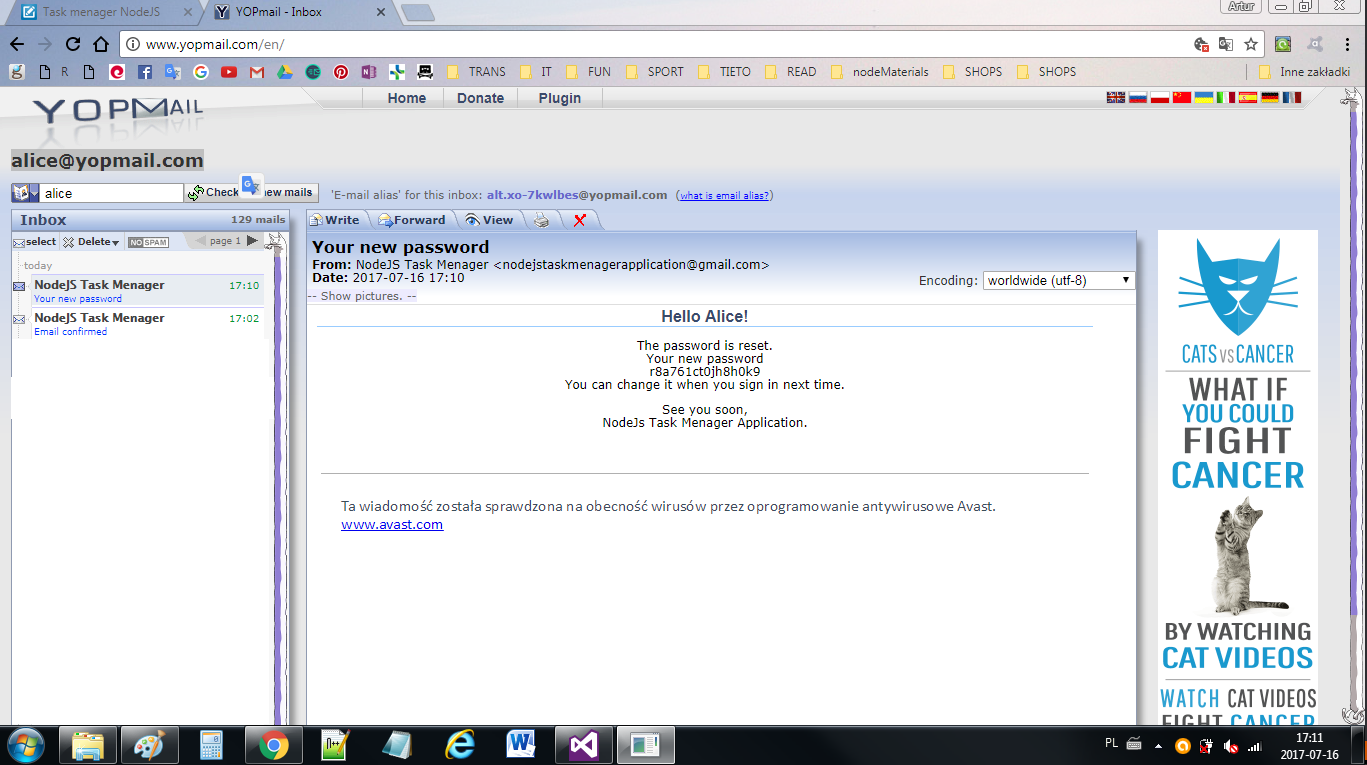
\includegraphics[width=\textwidth,height=\textheight,keepaspectratio]{53.png}
\captionsetup{labelformat=empty}
\caption[]{Otrzymujemy także wiadomość email zawierającą nowe hasło do serwisu.}
\end{figure}


\section{Zmiana danych użytkownika}
\begin{figure}[!hb]
\centering
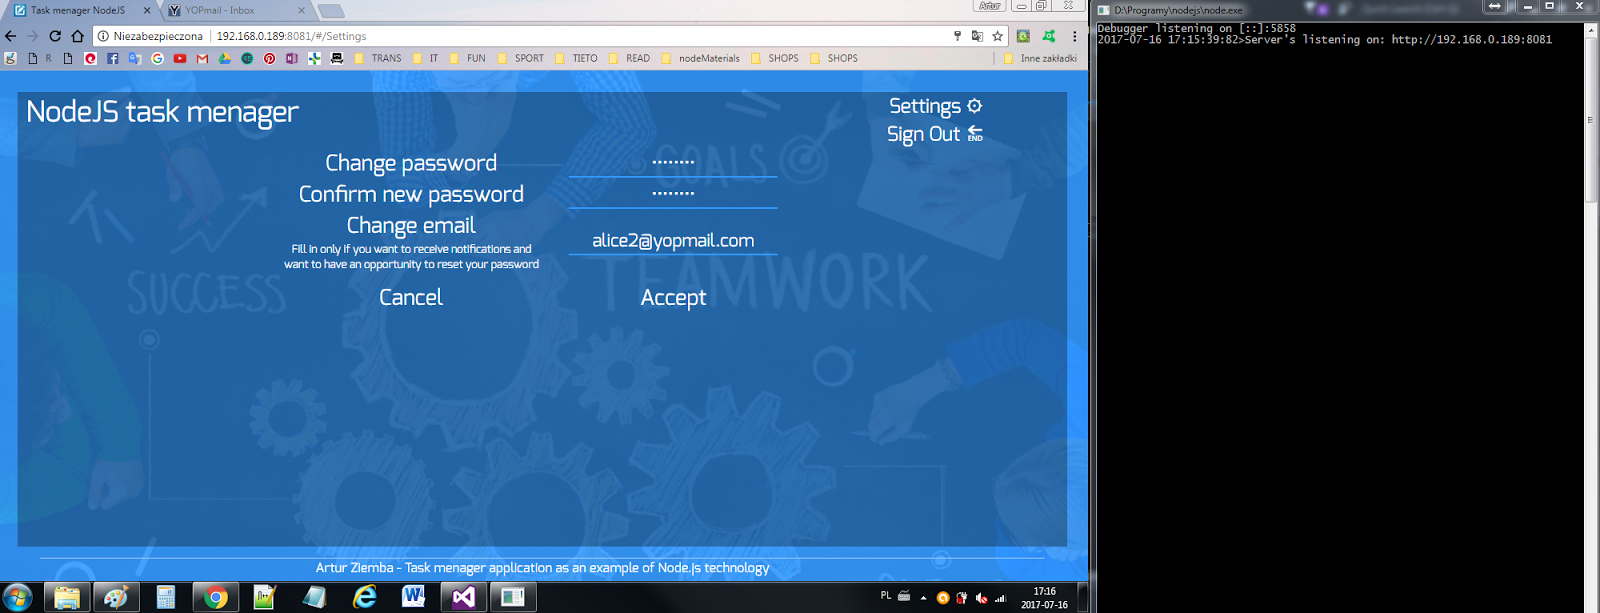
\includegraphics[width=\textwidth,height=\textheight,keepaspectratio]{61.png}
\captionsetup{labelformat=empty}
\caption[]{Po zalogowaniu się i wypełnieniu odpowiedniego formularza na stronie serwisu użytkownik wysyła żądanie do serwera.}
\end{figure}
\begin{figure}[!hb]
\centering
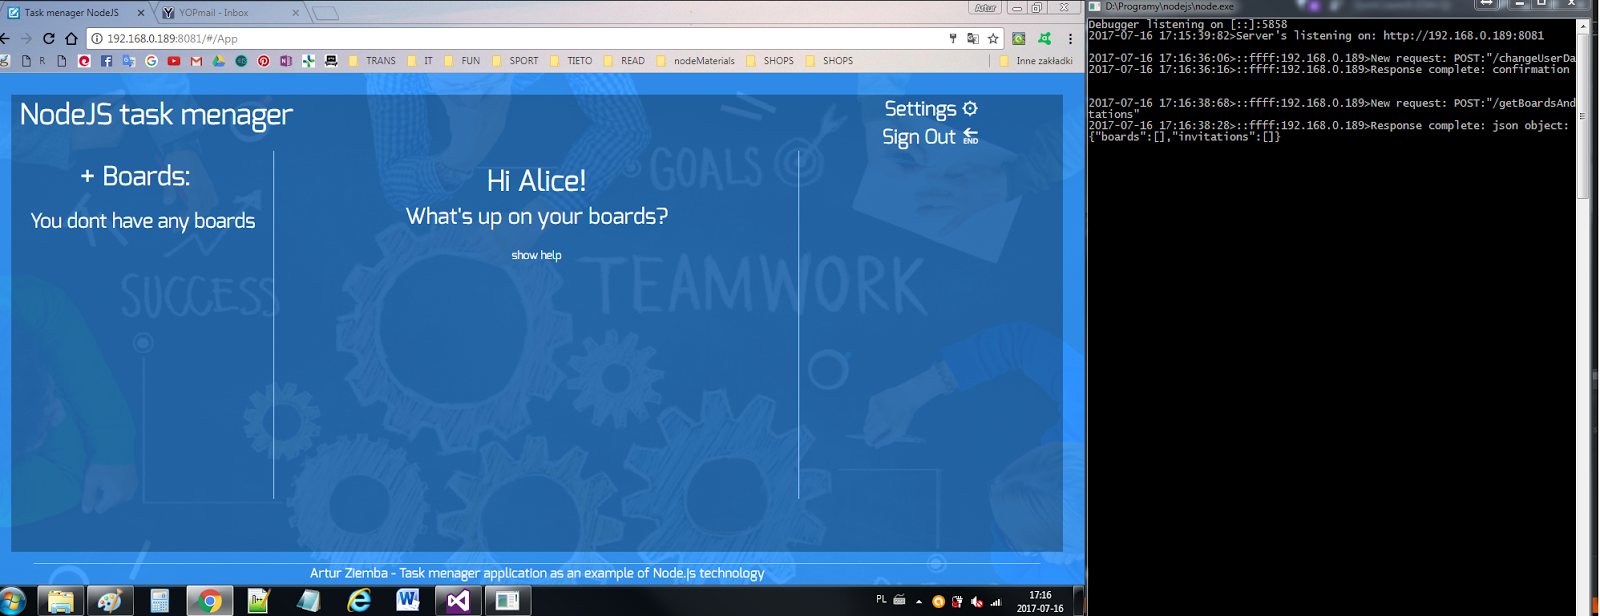
\includegraphics[width=\textwidth,height=\textheight,keepaspectratio]{62.png}
\captionsetup{labelformat=empty}
\caption[]{Serwer sprawdza poprawność danych. Jeśli są poprawne aktualizuje je.
W przeciwnym wypadku zwraca komunikat o błędzie. 
W odpowiedzi serwer wysyła strone główną aplikacji.}
\end{figure}
\begin{figure}[!hb]
\centering
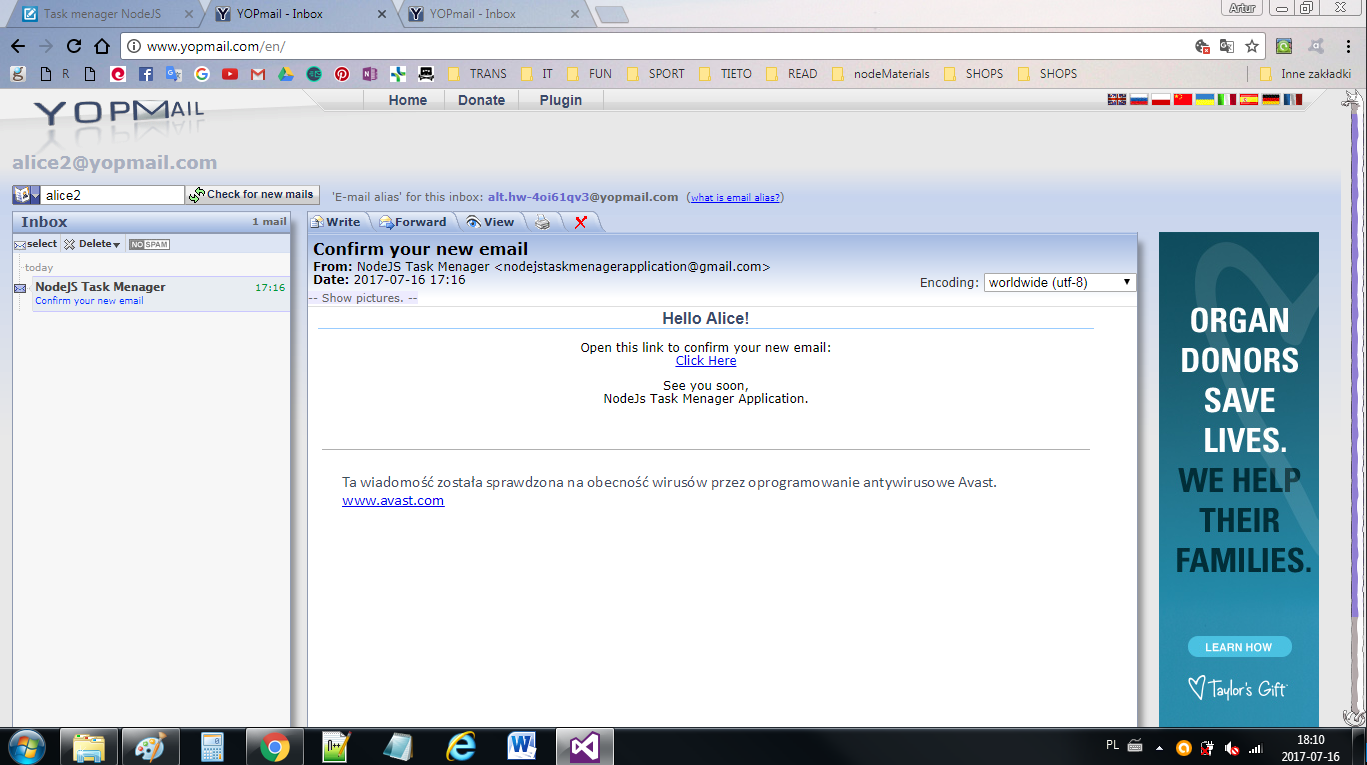
\includegraphics[width=\textwidth,height=\textheight,keepaspectratio]{63.png}
\captionsetup{labelformat=empty}
\caption[]{Jeśli zmieni się również adres email użytkownik musi go ponownie zweryfikowac. }
\end{figure}


\section{Utworzenie nowej tablicy z zadaniami}
\begin{figure}[!hb]
\centering
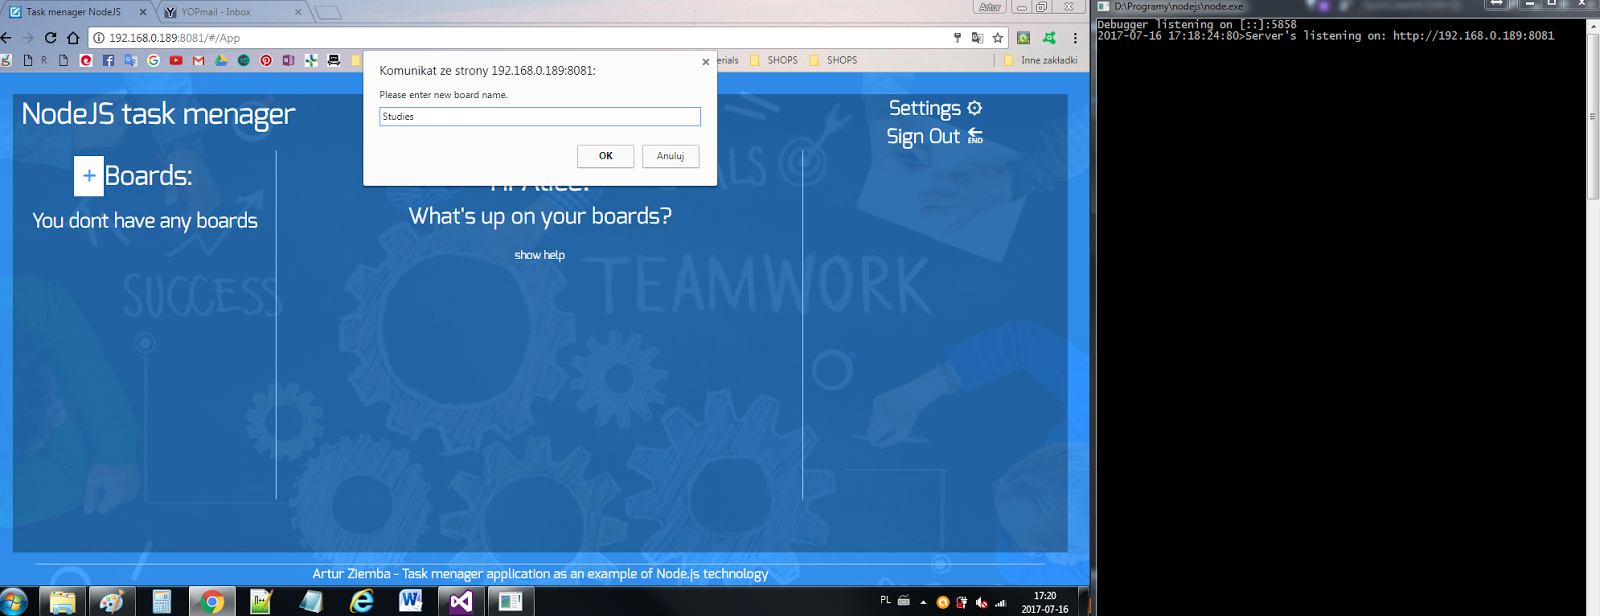
\includegraphics[width=\textwidth,height=\textheight,keepaspectratio]{71.png}
\captionsetup{labelformat=empty}
\caption[]{Po zalogowaniu się użytkownik wybiera opcje dodania tablicy, wpisuje wymagane dane i wysyła je do serwera.}
\end{figure}
\begin{figure}[!hb]
\centering
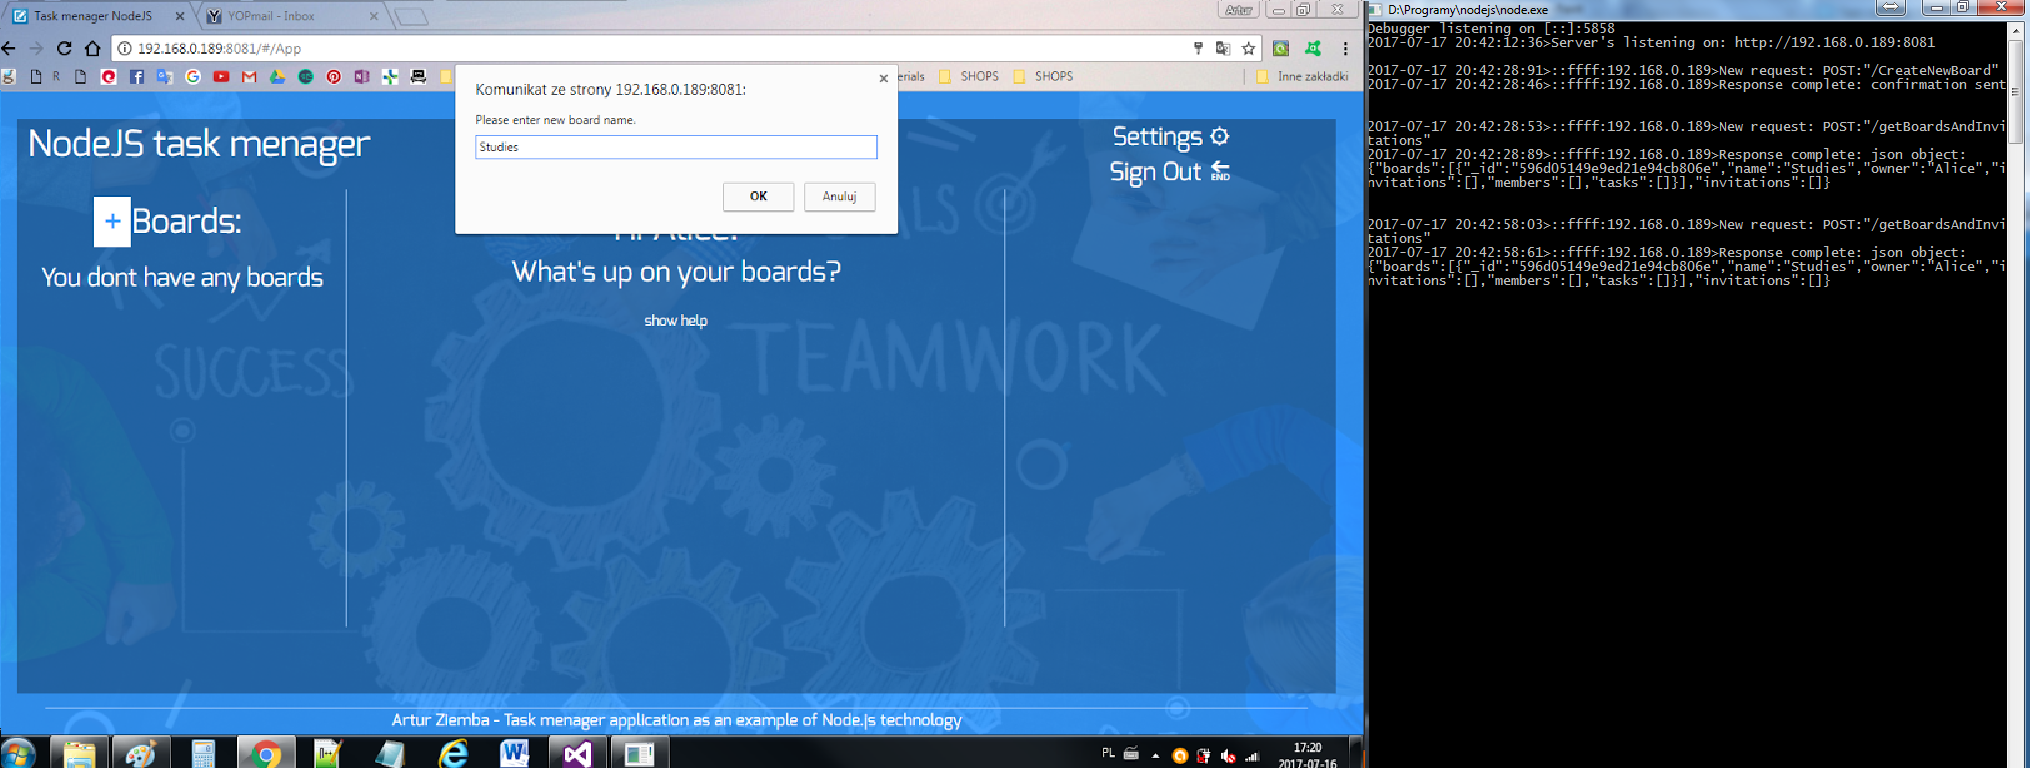
\includegraphics[width=\textwidth,height=\textheight,keepaspectratio]{72.png}
\captionsetup{labelformat=empty}
\caption[]{Serwer sprawdza poprawność danych. 
Jeśli są poprawne serwer tworzy nową tablice dla użytkownika i wysyła potwierdzenie w odpowiedzi.
W przeciwnym wypadku odpowiada komunikatem o błędzie.}
\end{figure}


\section{Wysyłanie zaproszenia do tablicy}
\begin{figure}[!hb]
\centering
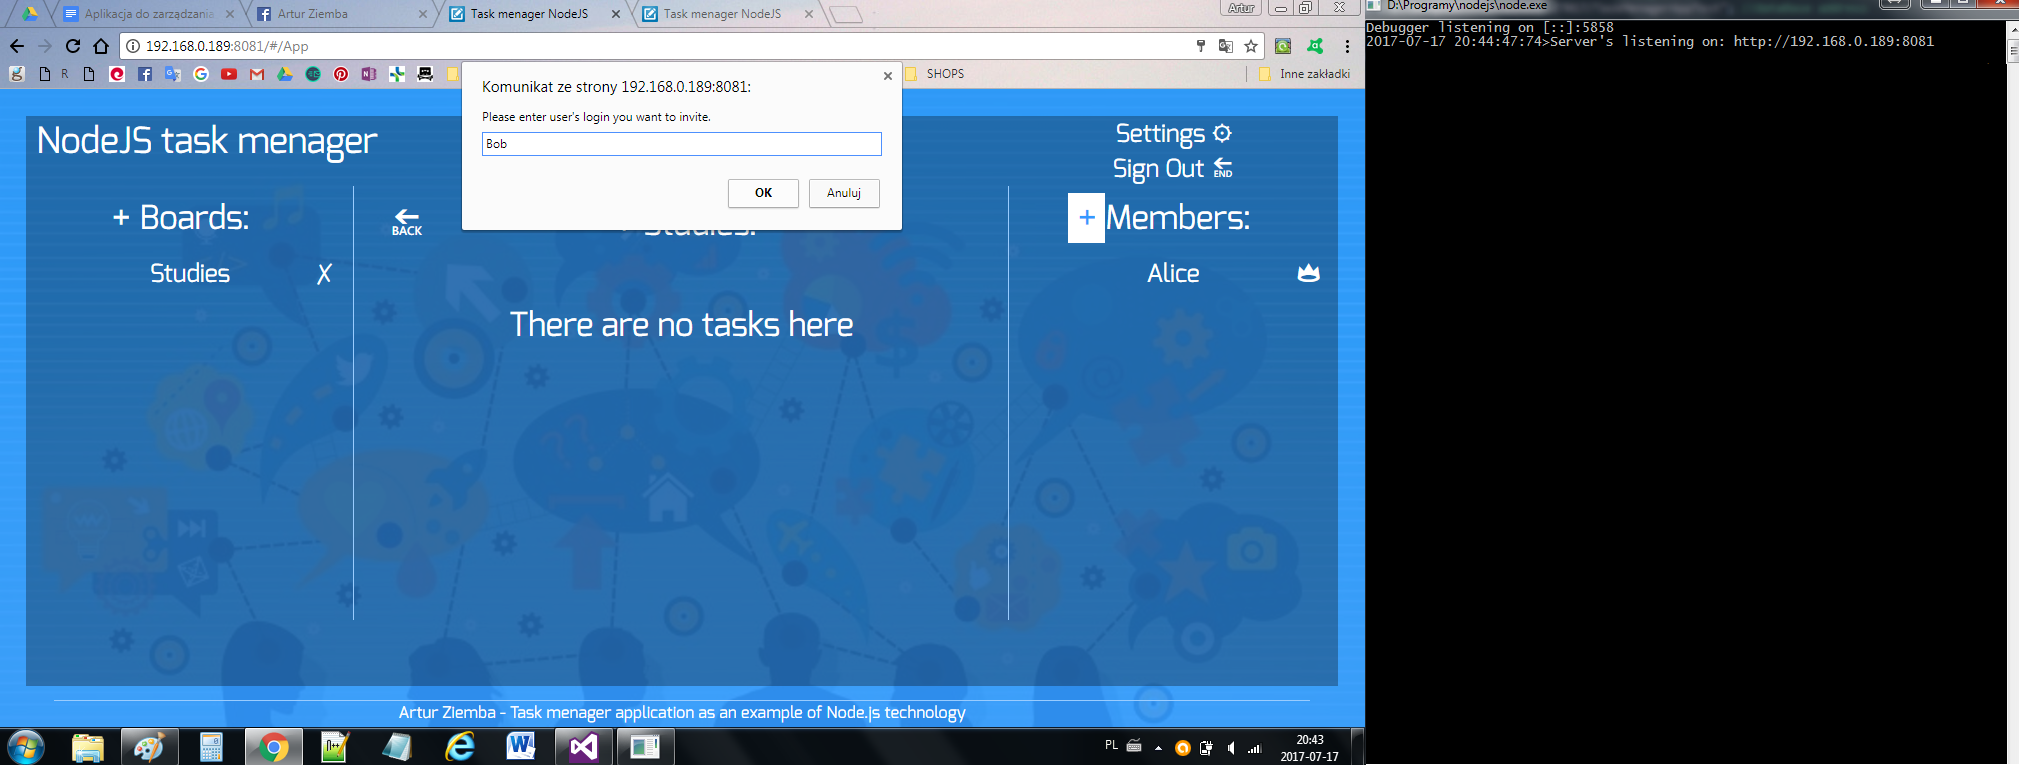
\includegraphics[width=\textwidth,height=\textheight,keepaspectratio]{01.png}
\captionsetup{labelformat=empty}
\caption[]{Po zalogowaniu się użytkownik wybiera opcje wysłania zaproszenia do wybranej tablicy, wypełnia dane i wysyła żądanie do serwera.}
\end{figure}
\begin{figure}[!hb]
\centering
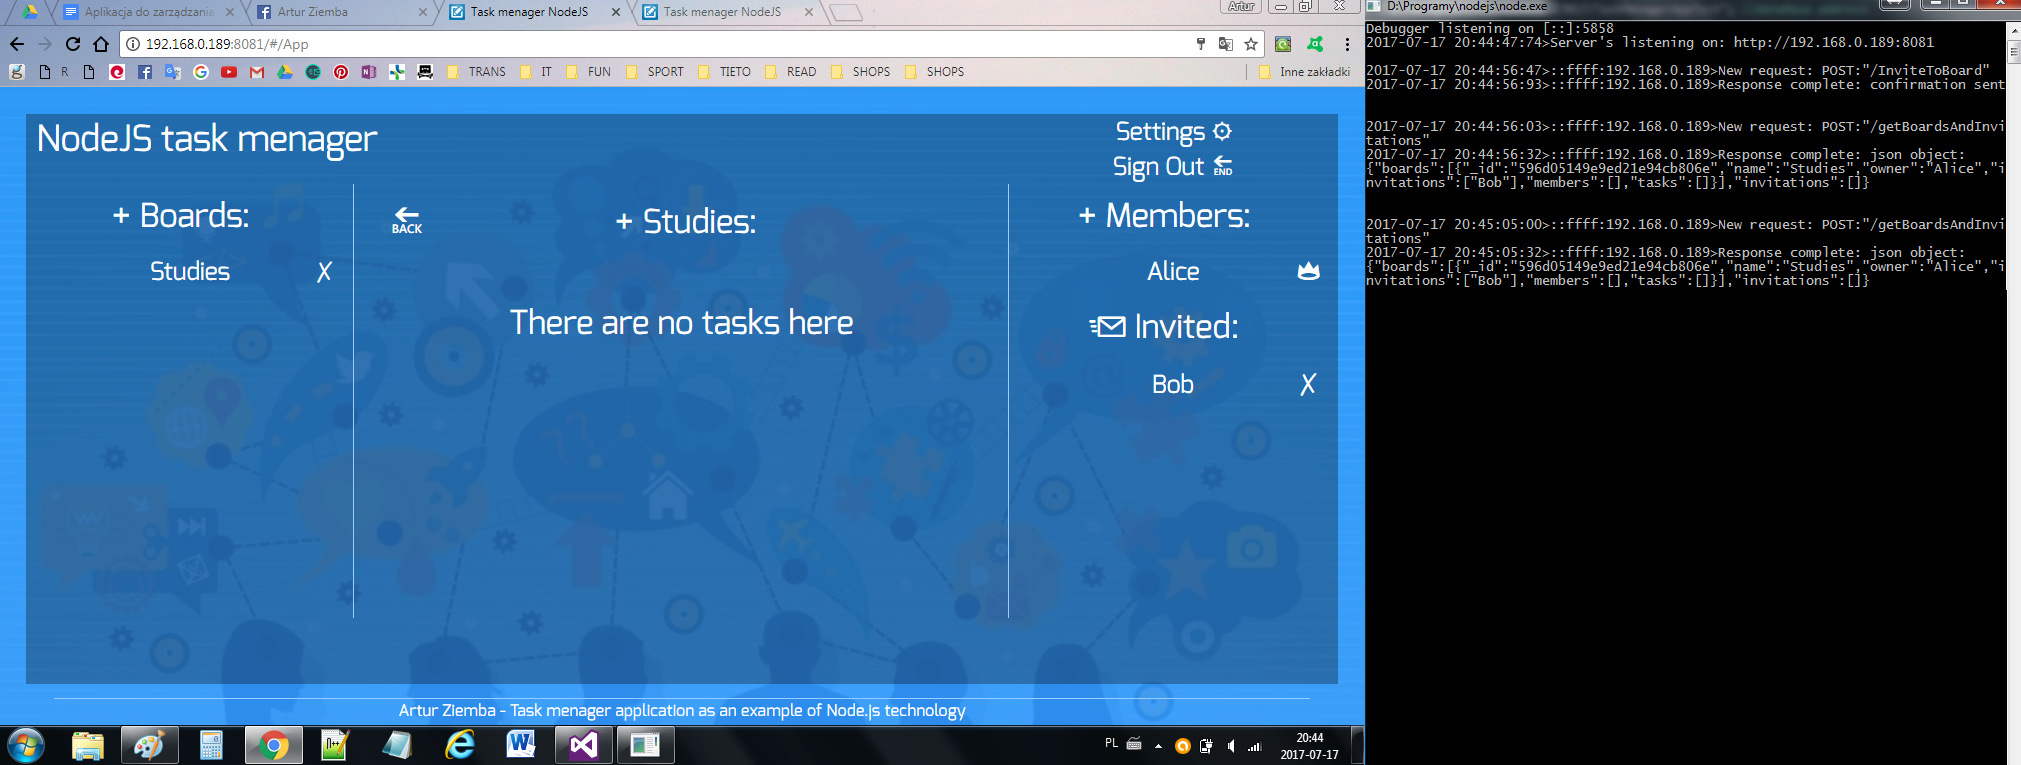
\includegraphics[width=\textwidth,height=\textheight,keepaspectratio]{02.png}
\captionsetup{labelformat=empty}
\caption[]{Serwer sprawdza poparwność danych. 
W odpowiedzi wysyła potwierdzenie o wysłanym zaproszeniu, lub komunikat o błędzie.}
\end{figure}


\section{Akceptacja zaproszenia}
\begin{figure}[!hb]
\centering
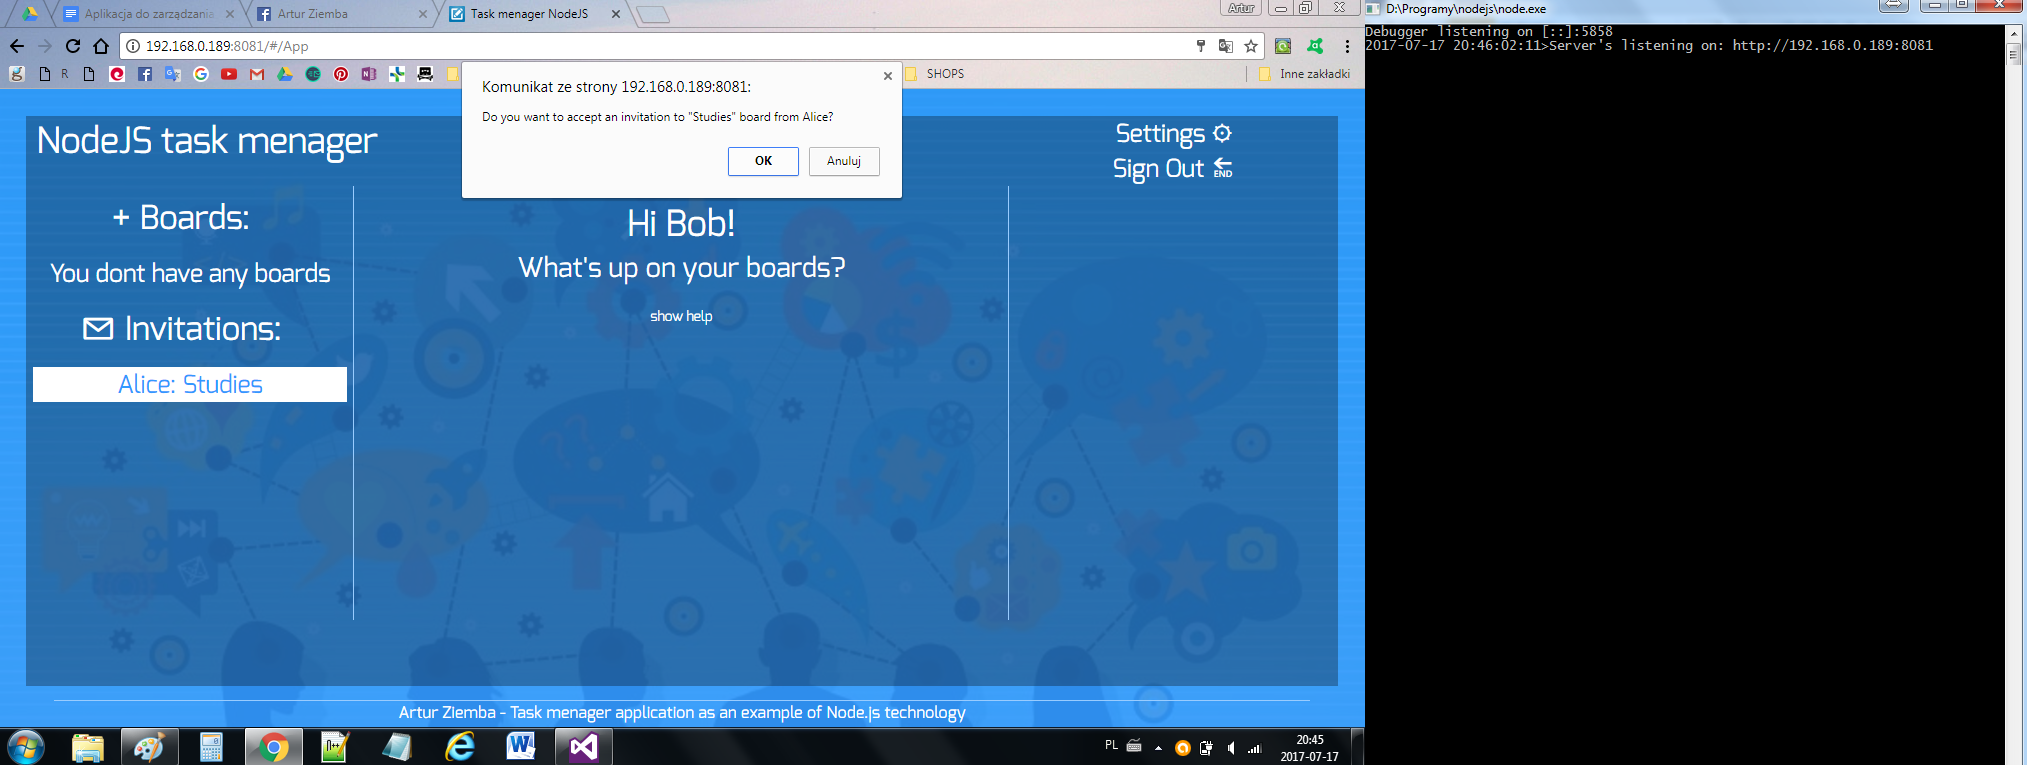
\includegraphics[width=\textwidth,height=\textheight,keepaspectratio]{81.png}
\captionsetup{labelformat=empty}
\caption[]{Po zalogowaniu się użytkownik wybiera opcje zaakceptowania oczekującego zaproszenia i wysyła żądanie do serwera.}
\end{figure}
\begin{figure}[!hb]
\centering
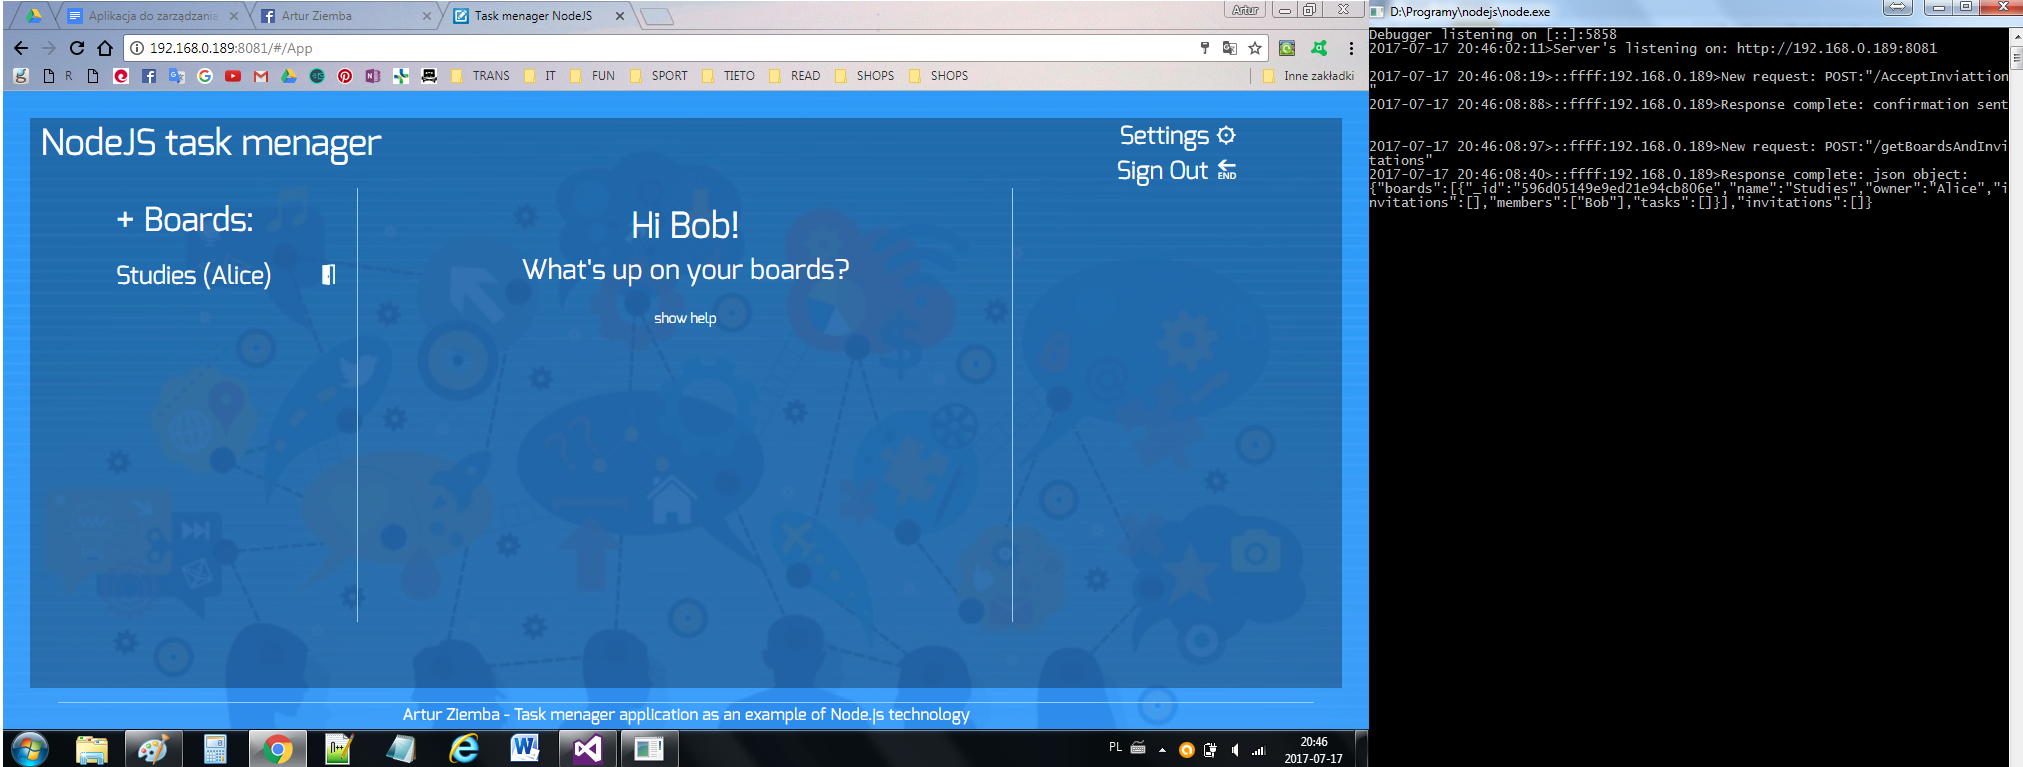
\includegraphics[width=\textwidth,height=\textheight,keepaspectratio]{82.png}
\captionsetup{labelformat=empty}
\caption[]{Serwer sprawdza poprawność danych. Odpowiada potwierdzeniem lub komunikatem o błędzie.}
\end{figure}


\section{Odrzucenie zaproszenia}
\begin{figure}[!hb]
\centering
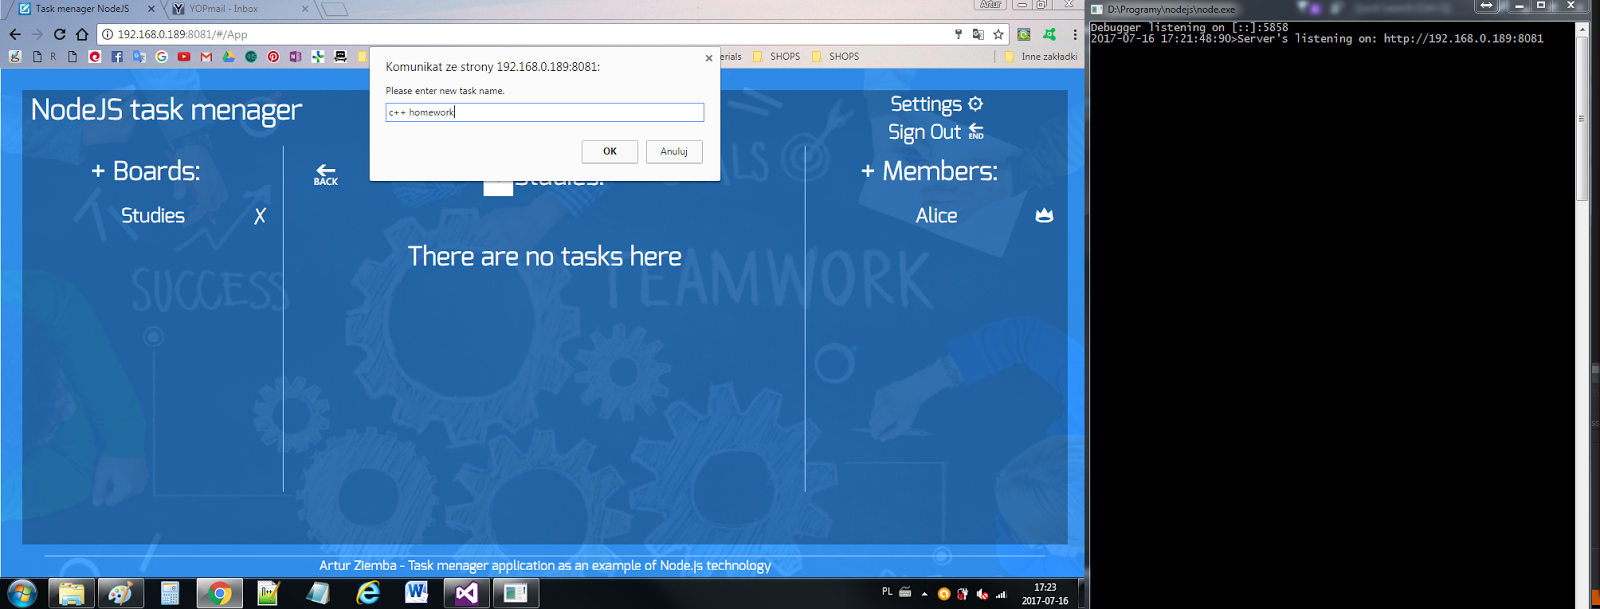
\includegraphics[width=\textwidth,height=\textheight,keepaspectratio]{A1.png}
\captionsetup{labelformat=empty}
\caption[]{Po zalogowaniu się użytkownik wybiera opcje odrzucenia oczekującego zaproszenia i wysyła żądanie do serwera.}
\end{figure}
\begin{figure}[!hb]
\centering
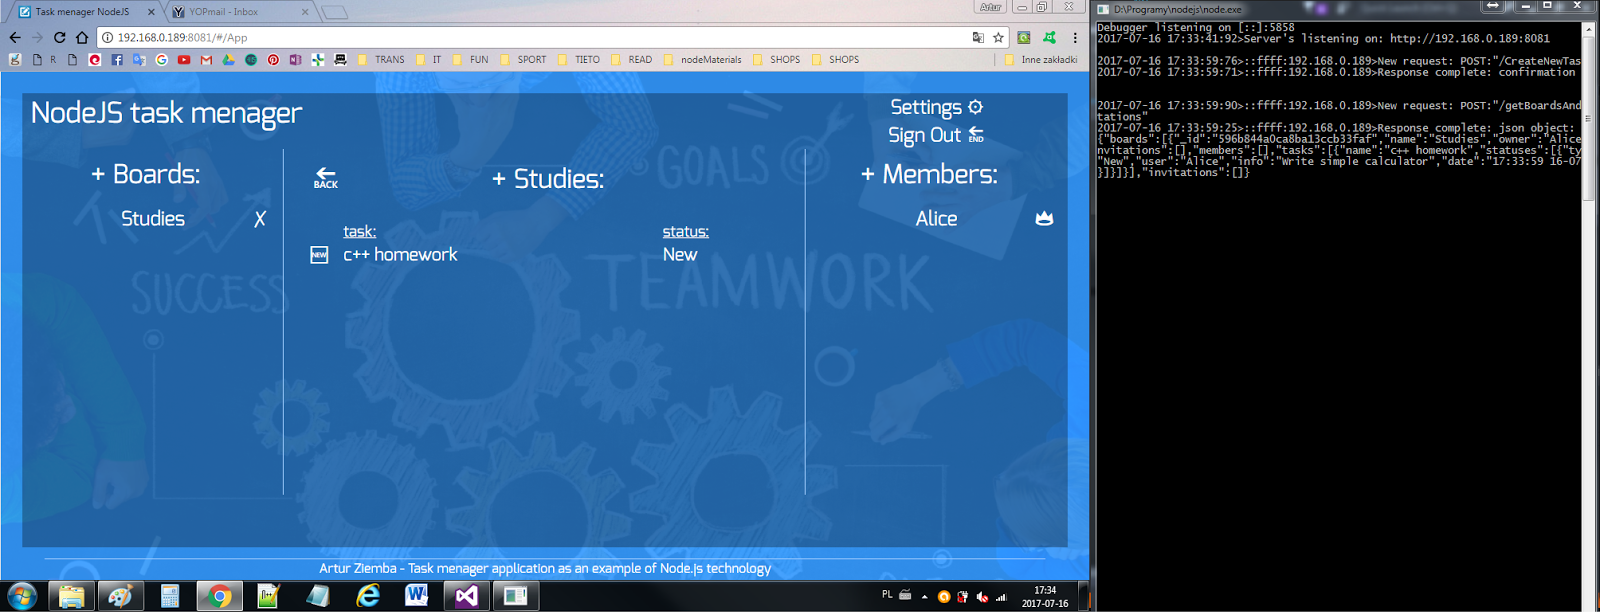
\includegraphics[width=\textwidth,height=\textheight,keepaspectratio]{A2.png}
\captionsetup{labelformat=empty}
\caption[]{Serwer sprawdza poprawność danych. Odpowiada potwierdzeniem lub komunikatem o błędzie.}
\end{figure}


\section{Wyrzucenie użytkownika z tablicy}
\begin{figure}[!hb]
\centering
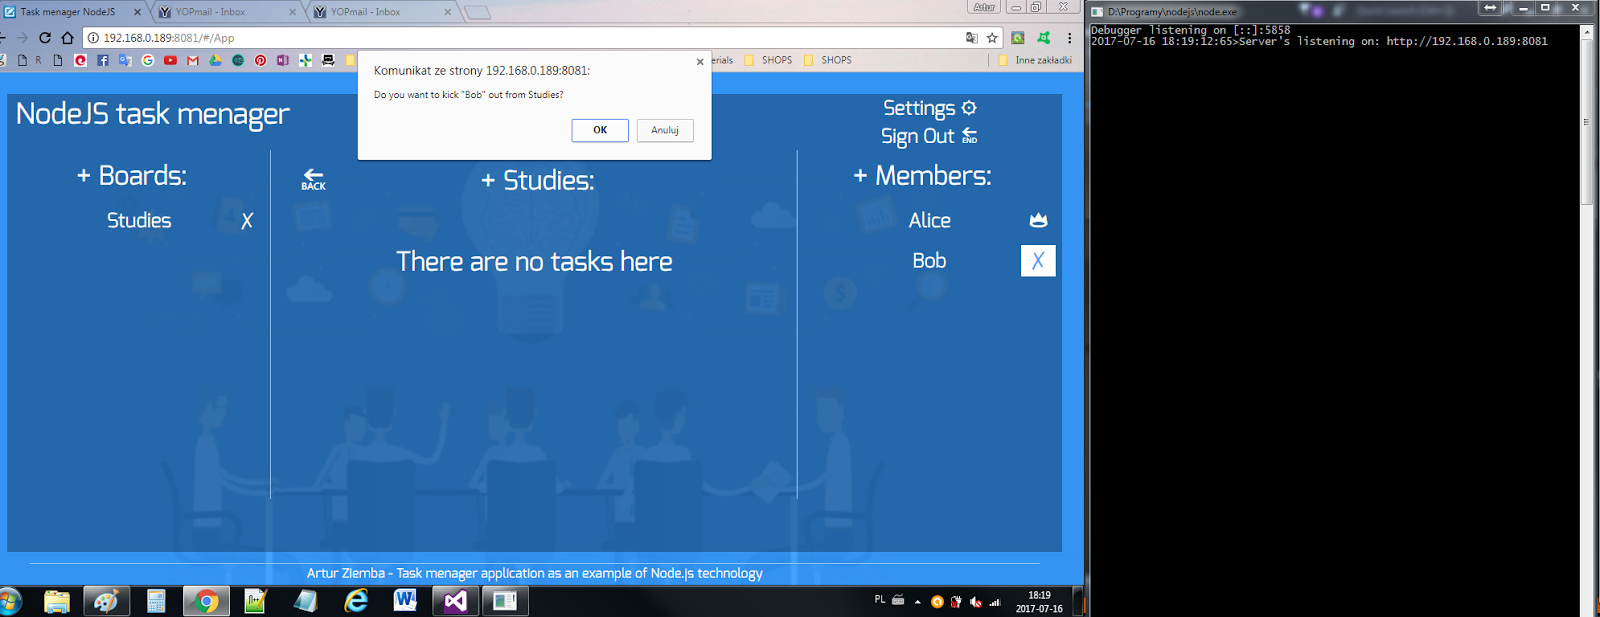
\includegraphics[width=\textwidth,height=\textheight,keepaspectratio]{91.png}
\captionsetup{labelformat=empty}
\caption[]{Po zalogowaniu się użytkownik wybiera opcje wyrzucenia użytkownika z określonej tablicy i wysyła żądanie do serwera.}
\end{figure}
\begin{figure}[!hb]
\centering
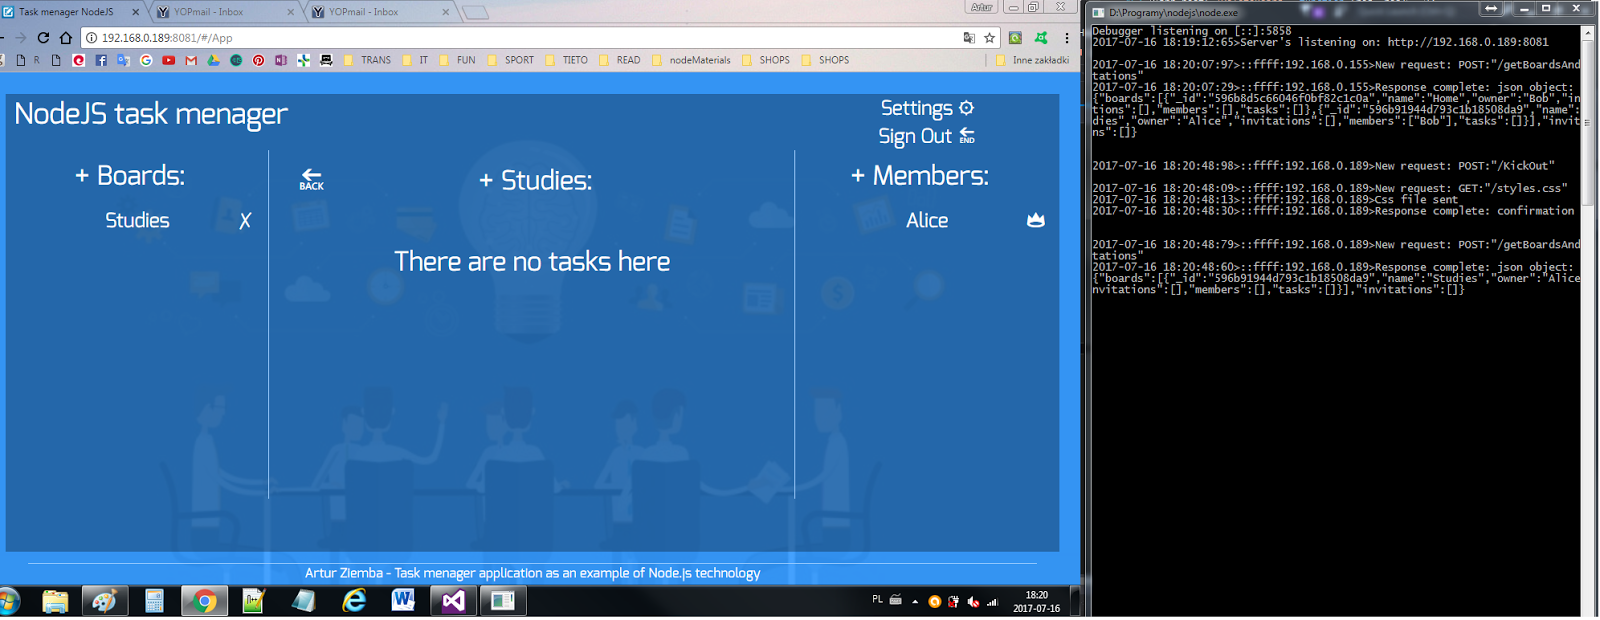
\includegraphics[width=\textwidth,height=\textheight,keepaspectratio]{92.png}
\captionsetup{labelformat=empty}
\caption[]{Serwer sprawdza poprawność danych. Odpowiada potwierdzeniem lub komunikatem o błędzie.}
\end{figure}


\section{Dodanie zadania}
\begin{figure}[!hb]
\centering
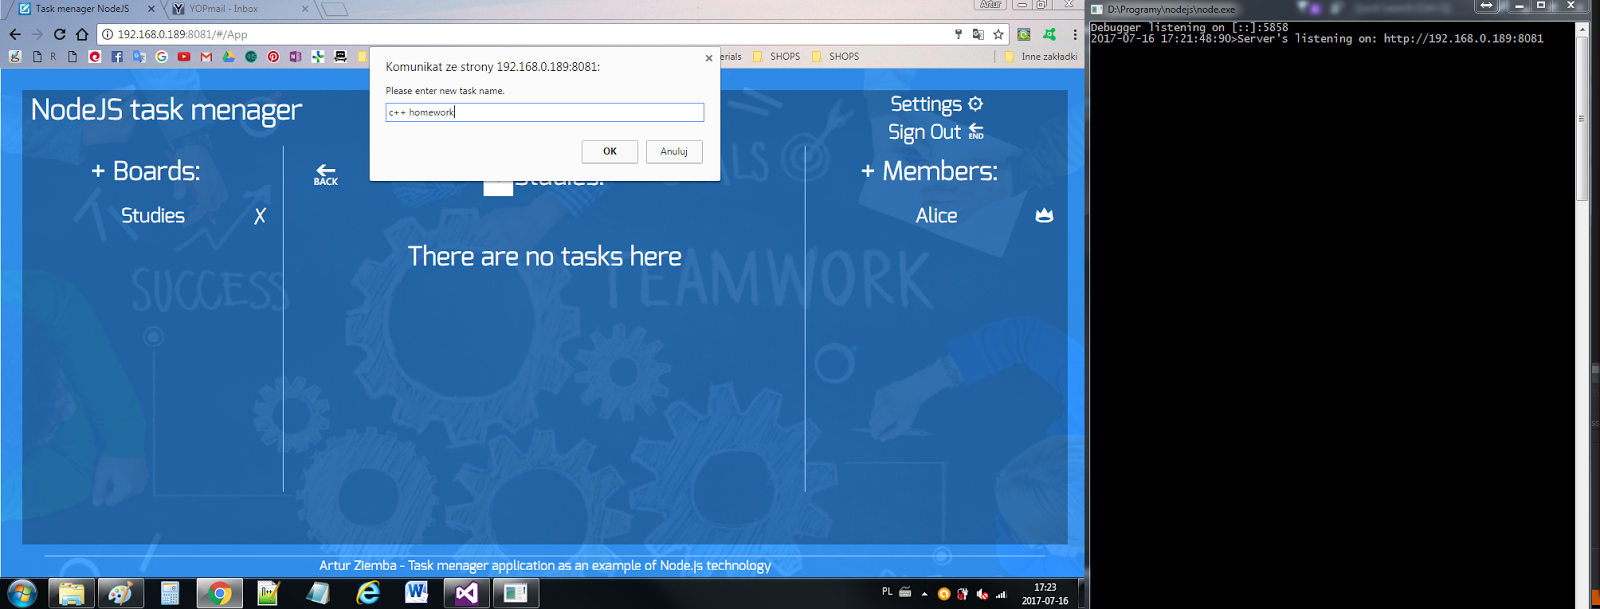
\includegraphics[width=\textwidth,height=\textheight,keepaspectratio]{A1.png}
\captionsetup{labelformat=empty}
\caption[]{Po zalogowaniu i wybraniu odpowiedniej tablicy użytkownik wybiera opcje dodania zadania, wypelnia dane i przesyła żądanie do serwera.}
\end{figure}
\begin{figure}[!hb]
\centering
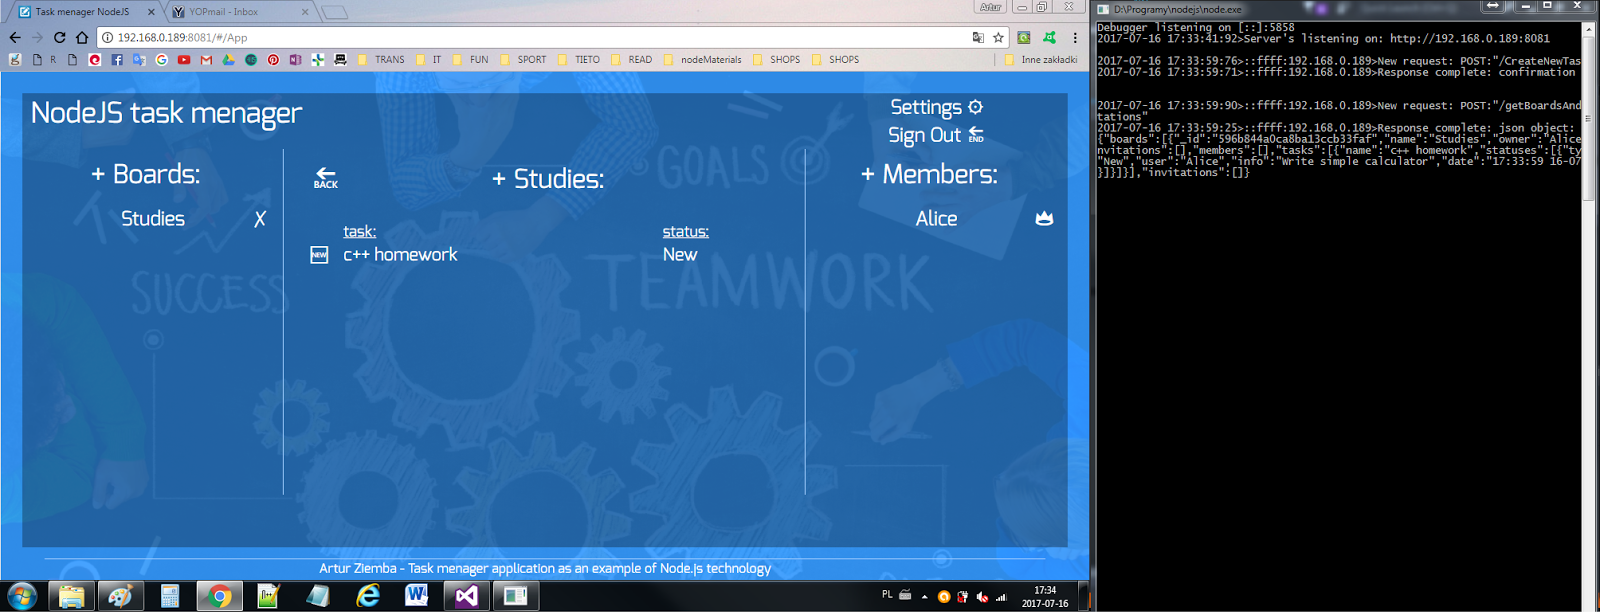
\includegraphics[width=\textwidth,height=\textheight,keepaspectratio]{A2.png}
\captionsetup{labelformat=empty}
\caption[]{Serwer sprawdza poprawność danych. Odpowiada potwierdzeniem lub komunikatem o błędzie.}
\end{figure}


\section{Dodanie statusu zadania}
\begin{figure}[!hb]
\centering
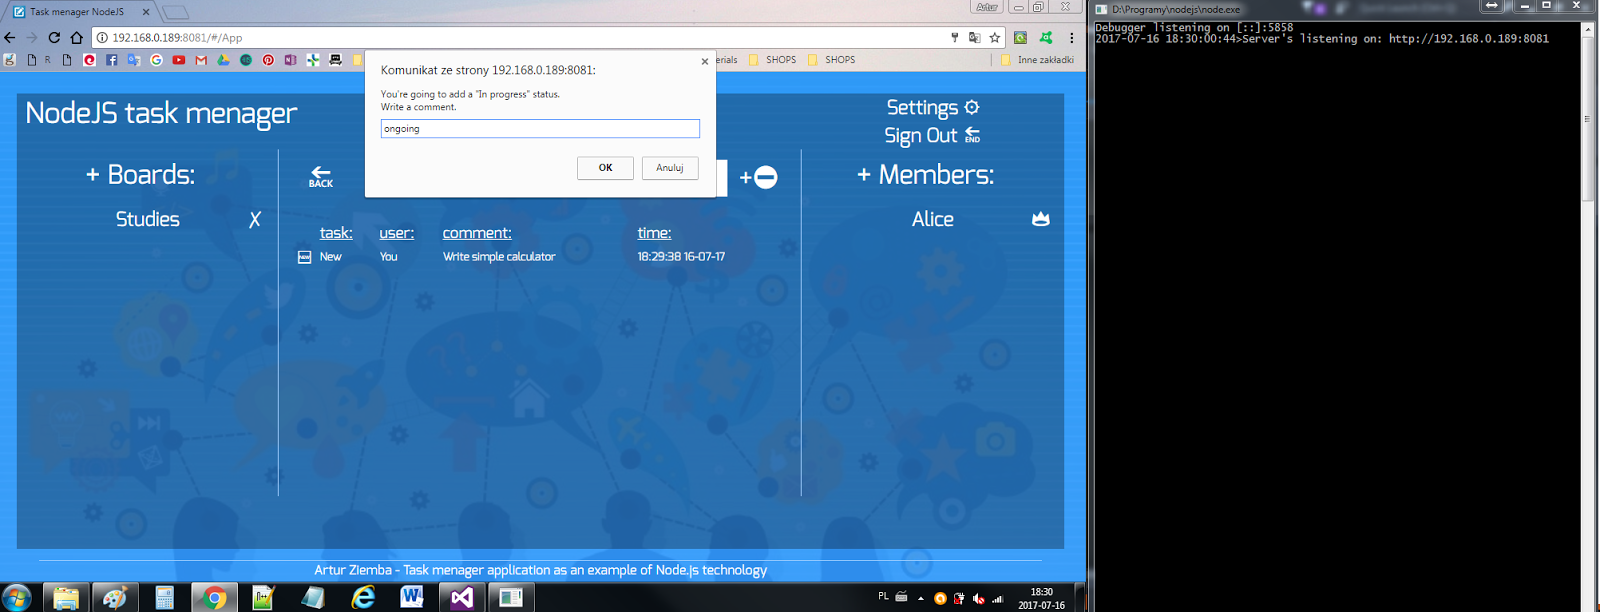
\includegraphics[width=\textwidth,height=\textheight,keepaspectratio]{B1.png}
\captionsetup{labelformat=empty}
\caption[]{Po zalogowaniu, wybraniu odpowiedniej tablicy i zadania użytkownik wybiera opcje dodania nowego statusu, uzupełnia dane i przesyła żądanie do serwera.}
\end{figure}
\begin{figure}[!hb]
\centering
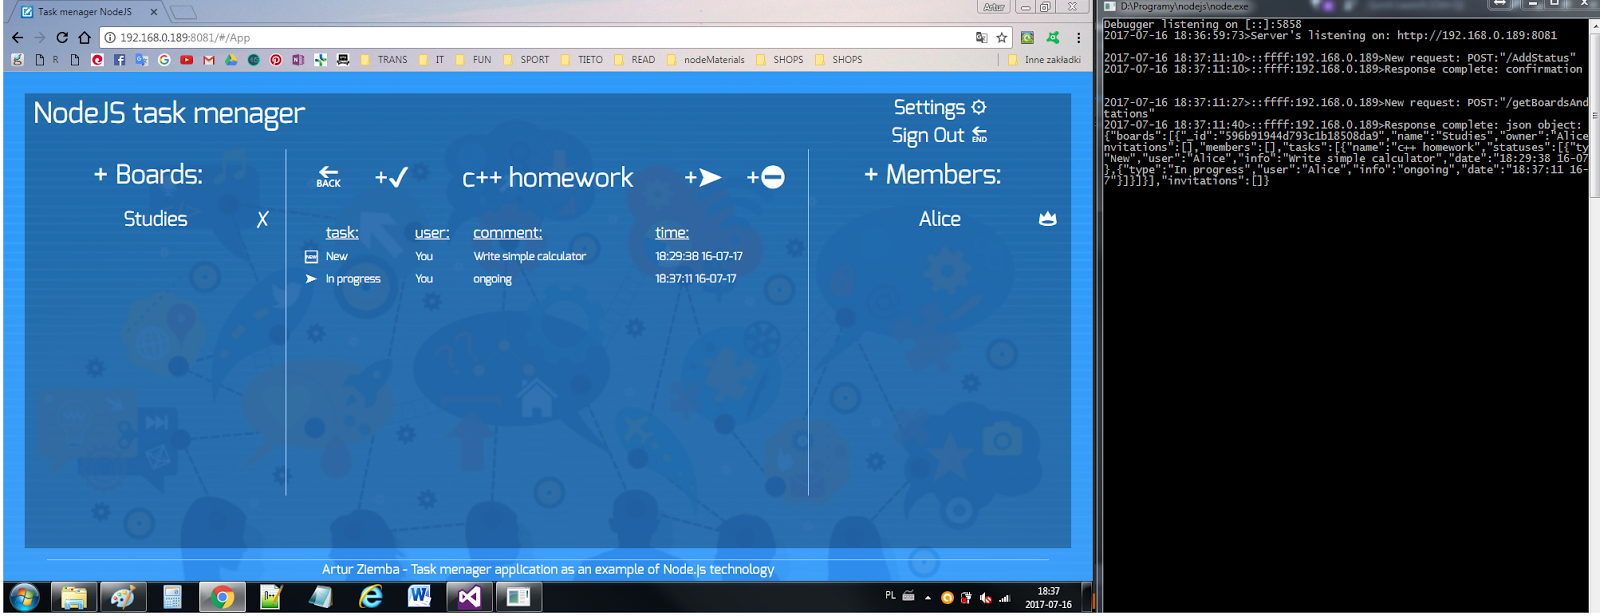
\includegraphics[width=\textwidth,height=\textheight,keepaspectratio]{B2.png}
\captionsetup{labelformat=empty}
\caption[]{Serwer sprawdza poprawność danych. Odpowiada potwierdzeniem lub komunikatem o błędzie.}
\end{figure}


\section{Usuwanie zadania}
\begin{figure}[!hb]
\centering
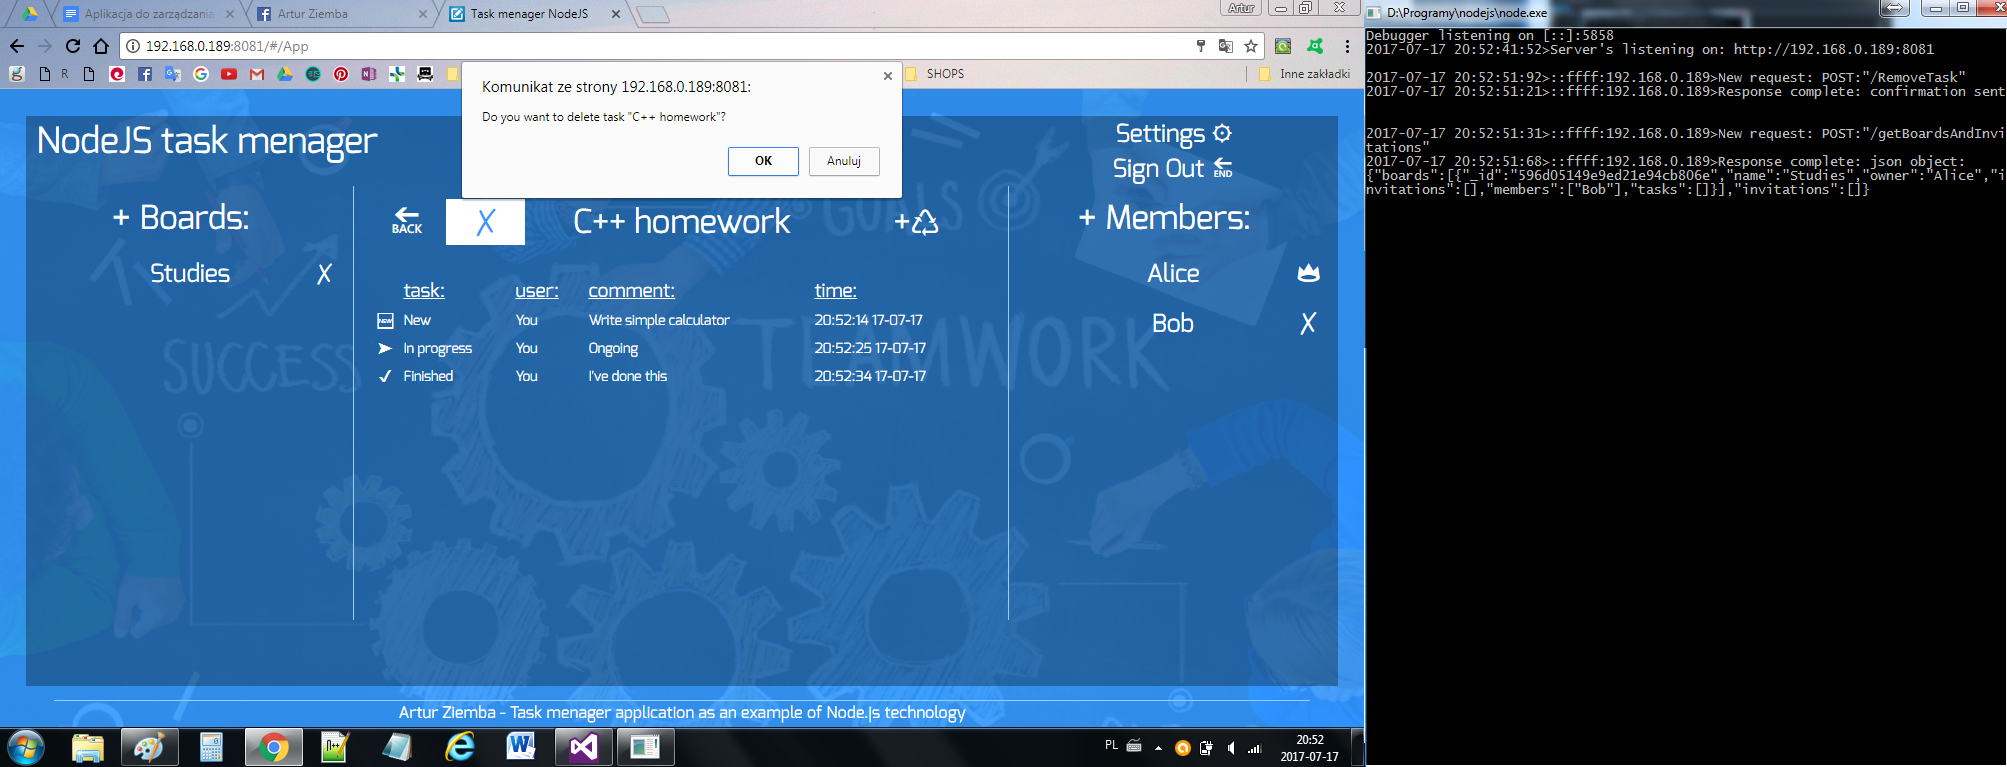
\includegraphics[width=\textwidth,height=\textheight,keepaspectratio]{C1.png}
\captionsetup{labelformat=empty}
\caption[]{Po zalogowaniu, wybraniu odpowiedniej tablicy i zakończonego zadania użytkownik wybiera opcje usuwania zadania i przesyła żądanie do serwera.}
\end{figure}
\begin{figure}[!hb]
\centering
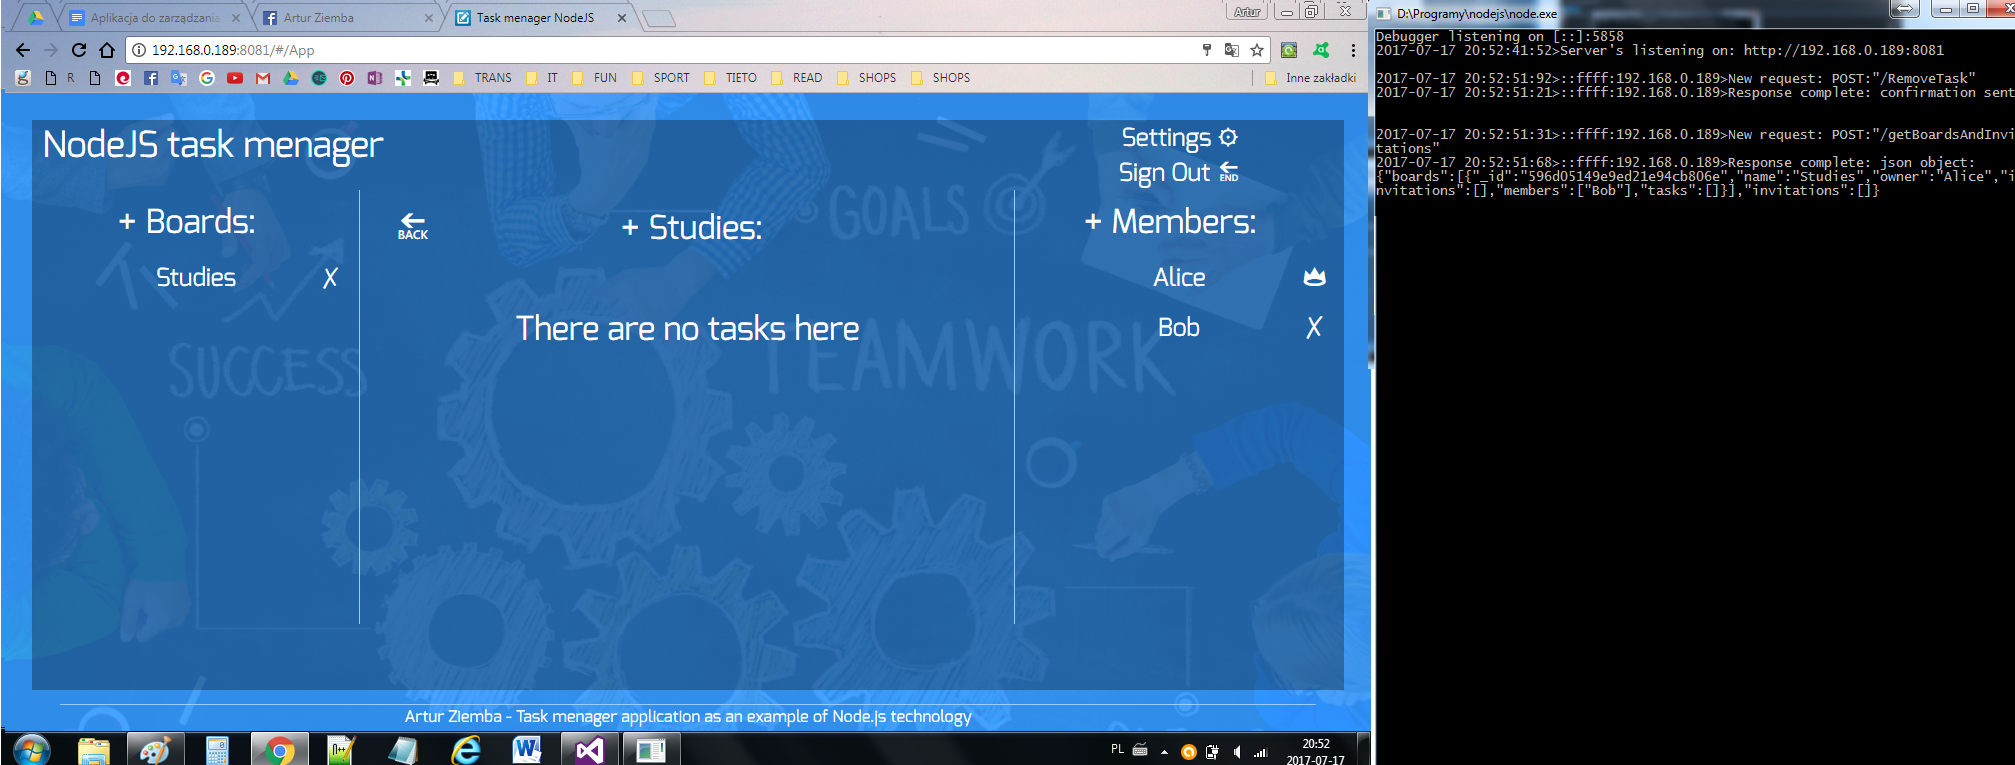
\includegraphics[width=\textwidth,height=\textheight,keepaspectratio]{C2.png}
\captionsetup{labelformat=empty}
\caption[]{Serwer sprawdza poprawność danych. Odpowiada potwierdzeniem lub komunikatem o błędzie.}
\end{figure}


\section{Opuszczanie tablicy}
\begin{figure}[!hb]
\centering
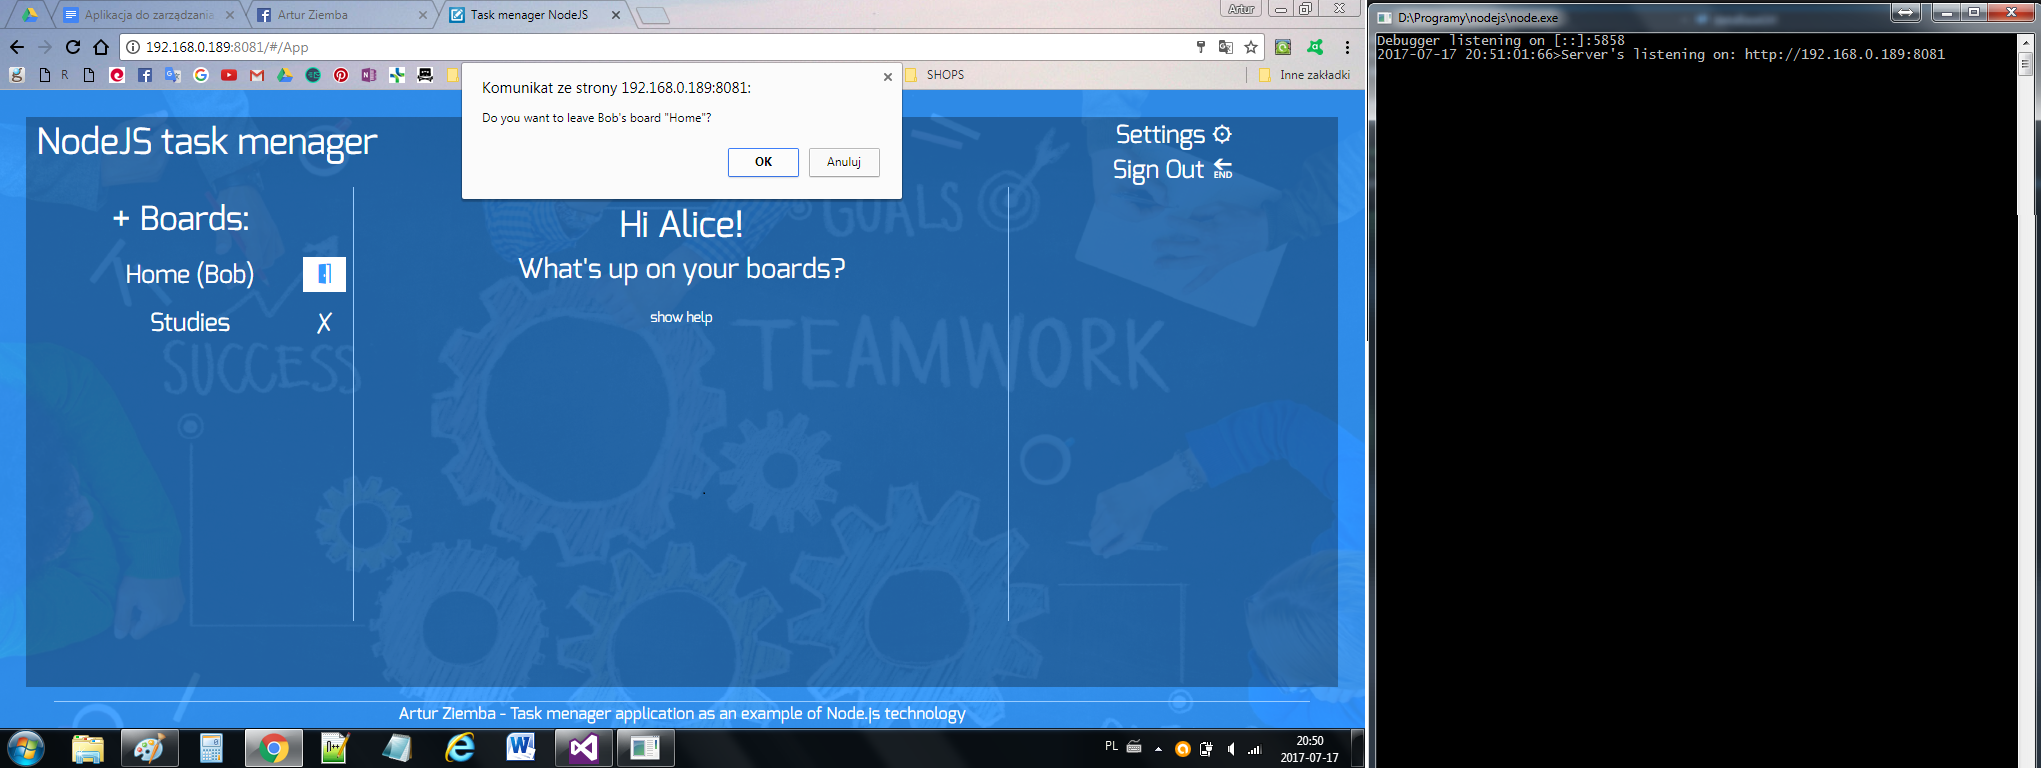
\includegraphics[width=\textwidth,height=\textheight,keepaspectratio]{D1.png}
\captionsetup{labelformat=empty}
\caption[]{Po zalogowaniu użytkownik wybiera opcje opuszczenia tablicy, której jest członkiem i wysyła żądanie do serwera.}
\end{figure}
\begin{figure}[!hb]
\centering
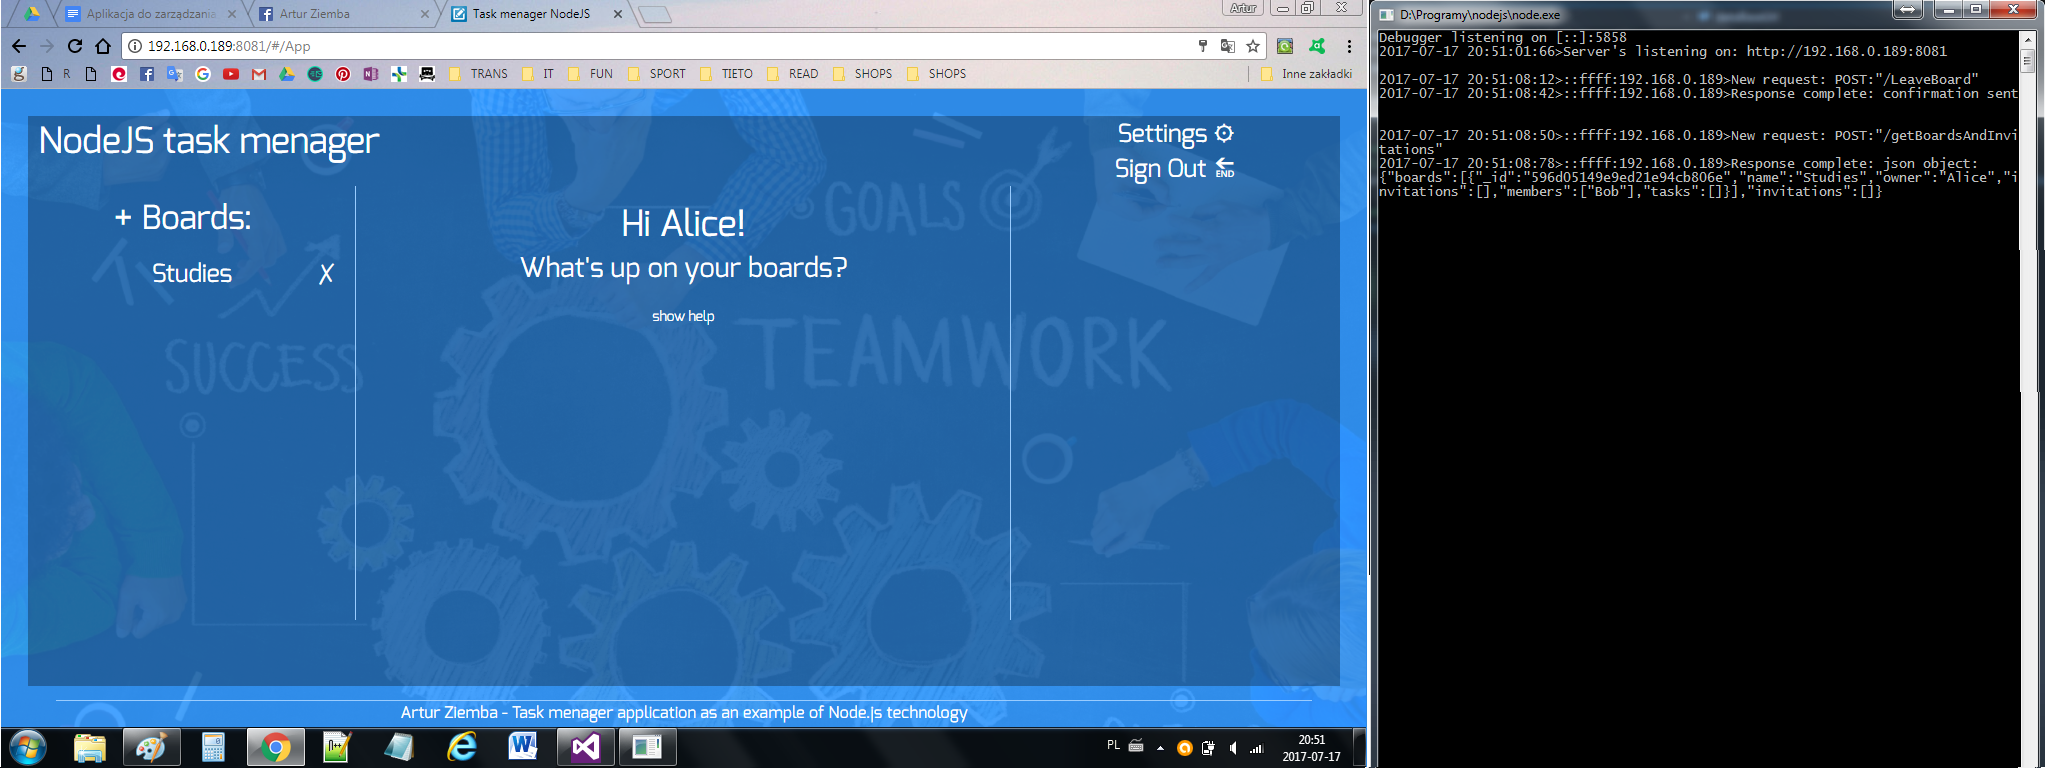
\includegraphics[width=\textwidth,height=\textheight,keepaspectratio]{D2.png}
\captionsetup{labelformat=empty}
\caption[]{Serwer sprawdza poprawność danych. Odpowiada potwierdzeniem lub komunikatem o błędzie.}
\end{figure}


\section{Usuwanie tablicy}
\begin{figure}[!hb]
\centering
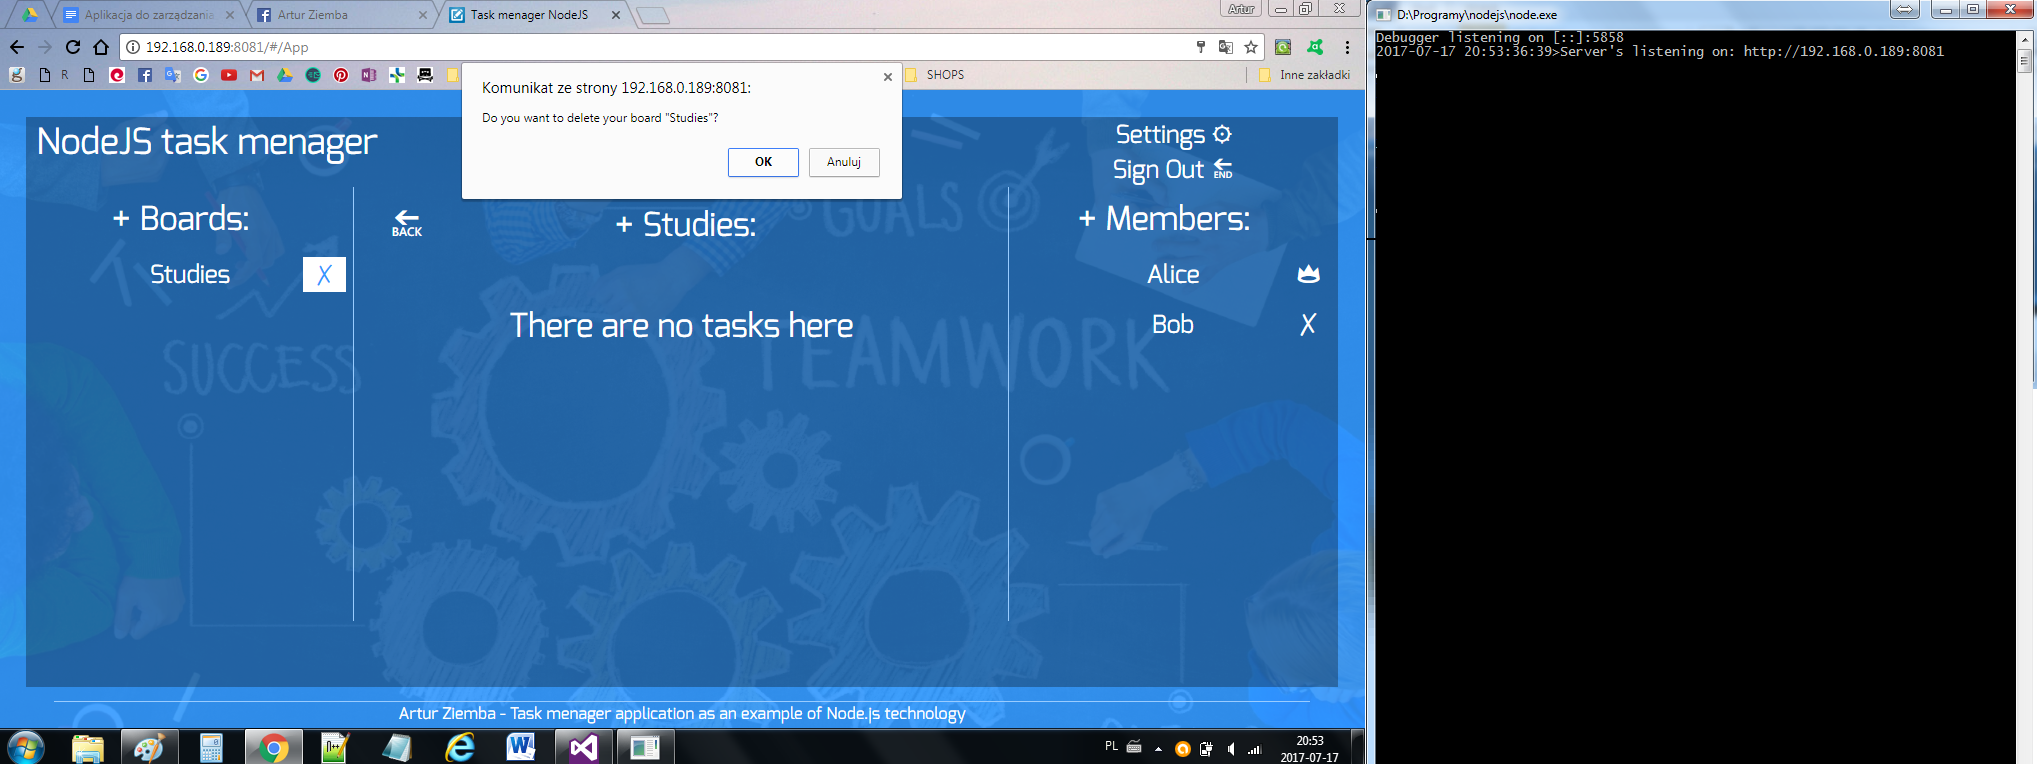
\includegraphics[width=\textwidth,height=\textheight,keepaspectratio]{E1.png}
\captionsetup{labelformat=empty}
\caption[]{Po zalogowaniu użytkownik wybiera opcje usunięcia własnej tablicy i wysyła żądanie do serwera.}
\end{figure}
\begin{figure}[!hb]
\centering
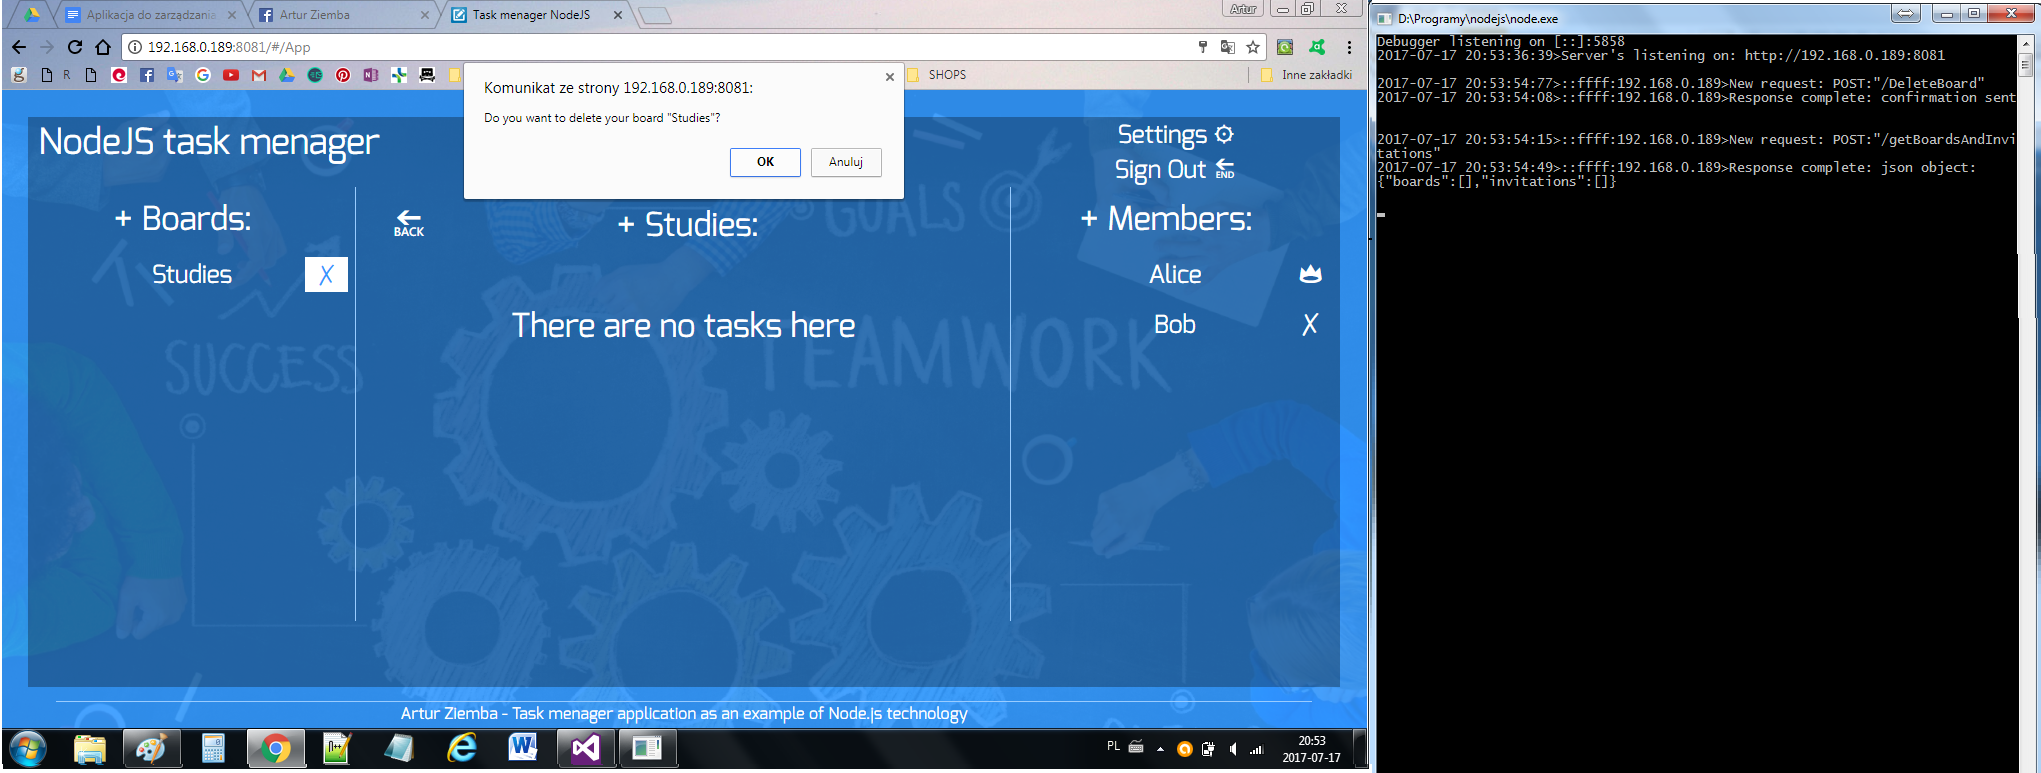
\includegraphics[width=\textwidth,height=\textheight,keepaspectratio]{E2.png}
\captionsetup{labelformat=empty}
\caption[]{Serwer sprawdza poprawność danych. Odpowiada potwierdzeniem lub komunikatem o błędzie.}
\end{figure}


\chapter{Podsumowanie otrzymanych wyników i wnioski na temat środowiska}
Wykoanana aplikacja spełnia zadana w warunkach funkcjonalność. 
Zostały osiągnięte wszystkie założenia oraz wymagania aplikacji przy użyciu możliwości dostarczanej przez technologie Node.js. 
Stworzony projekt doskonale nadaje się do użytkownia przez zorganizowane zespoły do wykonywania określonych zadań. 
Mógłby być na przykład używany do zarządzania pracą zespołów deweloperskich pracujących w różnych metodykach takich jak scrum czy kanban. 
Dostarcza przejrzysty interfejs oraz nieskomplikowaną prezętacje danych dla końcowych użytkowników, przez co nie wymaga praktycznie żadnych szkoleń lub procesów wdrożenioywch w celu zdobycia umiejętności biegłej obsługi narzędzia. 
Środowisko Node.js wydaje się być bardzo nowoczesnym oraz mającym przed sobą świetlana przyszlość środowiskiem. 
Niewątpliwie największymi zaletami tej technologii jest łatwość budowania wymagających serwisów internetowych poprzez użycie asynchronicznej obsługi wejścia/wyjścia, które pozwala na przetwarzanie wielu funkcji w jednym czasie tworząc wyjątkowo szybkie w działaniu aplikacje. 
Zagadnienie to wymaga jednak umiejętności w projektowaniu i analizowaniu funkcji programowania asynchronicznego. 
Kod pisany jest w szeroko używanym języku javaScript co zbudowało ogromną społeczność zainteresowaną technologią Node.js. 
Dzięki temu możemy z łatwością zdobyć materiały przydatne w procesie poznwaczym środowiska. 
Globalne repozytorium npm gwarantuje obsługe wielu funkcjonalności, bez potrzeby długiego szukania możliwych rozwiązań. 
Wszystko jest dostępne bezpłatnie, gotowe do wdrożenia w tworzonej aplikacji. 
Mimo że jest to technologia stosunkowo młoda obecnie Node.js jest używany, a co za tym idzie sprawdzony przez największe firmy IT w celu obsługi ich aplikacji i serwerów. 
Należy być świadomym wszytkich zalet i wad przy wyborze określonej technologii. 
Node.js nie nadaje się niestety do każdego typu projektu. 
Nie jest efektywnym środowiskiem jeśli chodzi o korzystanie z obliczeń intensywnie wykorzystujących procesor. 
Jest on jednak że idealnym rozwiązaniem w przypadku pracy nad wieloma rozwiązaniami webowymi. 
Osobiście praca w Node.js sprawiła mi wielką radość i stała się moją ulubioną technologią dzięki zapewnionej prostocie i możliwych do uzyskania bez większego wysiłku ogromnych możliwościach.

\addcontentsline{toc}{chapter}{Bibliografia} 
\begin{thebibliography}{99}
\bibitem{Brown} 
Ethan Brown
\textit{Web Development with Node and Express: Leveraging the JavaScript Stack 1st Edition ISBN: 9781491949306}
\bibitem{Onodi} 
Robert Onodi
\textit{MEAN Blueprints ISBN: 9781783553945}
\bibitem{Node.js} 
Dokumentacja języka programowania Node.js. Stan na dzień: 2017-07-20
\textit{https://Node.js.org/en/docs}

\end{thebibliography}

\addcontentsline{toc}{chapter}{Spis rysunków} 
\listoffigures

\end{document}
